\chap{Group Actions, with Applications }{actions}
We've defined a  ``group'' as as set with an operation defined on it.  From this point of view, group elements are ``objects'' in a set. We have many examples of this: like the integers with addition, the integers mod $n$, the group of units $U(n)$, groups of matrices, and so on.

Later on we introduced the idea that permutations form a group. Permutations are actually bijections (1-1, onto functions) that map a set of objects to itself.  Another way of saying this is that permutations ``act on'' a set by moving the elements around.  Similarly, we saw in Figure~\ref{groups_s3_symmetry_fig} in Section~\ref{SymmetryGroup} that the symmetries of an equilateral triangle (which are elements of the group $S_3$) move the vertices of the triangle from one position to another.  As a third example, in the group $\mathbb {Q}^*$ of non-zero rational numbers we can think of left multiplying by $2$ as ``moving''  $-5$ over to $-10$.  Left multiplying again by $2$ ``moves'' $-10$ to $-20$: and so on.   

The examples in the previous paragraph  illustrate a general concept called \emph{group actions}\index{Actions!group}. We will see in this chapter how group actions can give us deeper insight into the symmetries that we see in the world around us. In particular, we will focus on what group actions can tell us about regular polyhedra such as the tetrahedron and cube.
\bigskip

This chapter  is by Holly Webb, with numerous additions by Mark Leech. Thanks to Tom Judson for material used in this chapter.

\section{Basic definitions}\label{DefActions}
We'll get to definitions momentarily, but first it's helpful to look at an example.

\begin{example}{Actions1} Consider the group $S_3=\{id,(AB),(AC),(BC),(ABC),(ABC)\}$ and the set $X=\{A,B,C\}$. Each element of $S_3$ ``does something" to each element of $X$. See the Figure~\ref{fig:S3onABC} below.

\begin{figure}[htbp]
\begin{center}
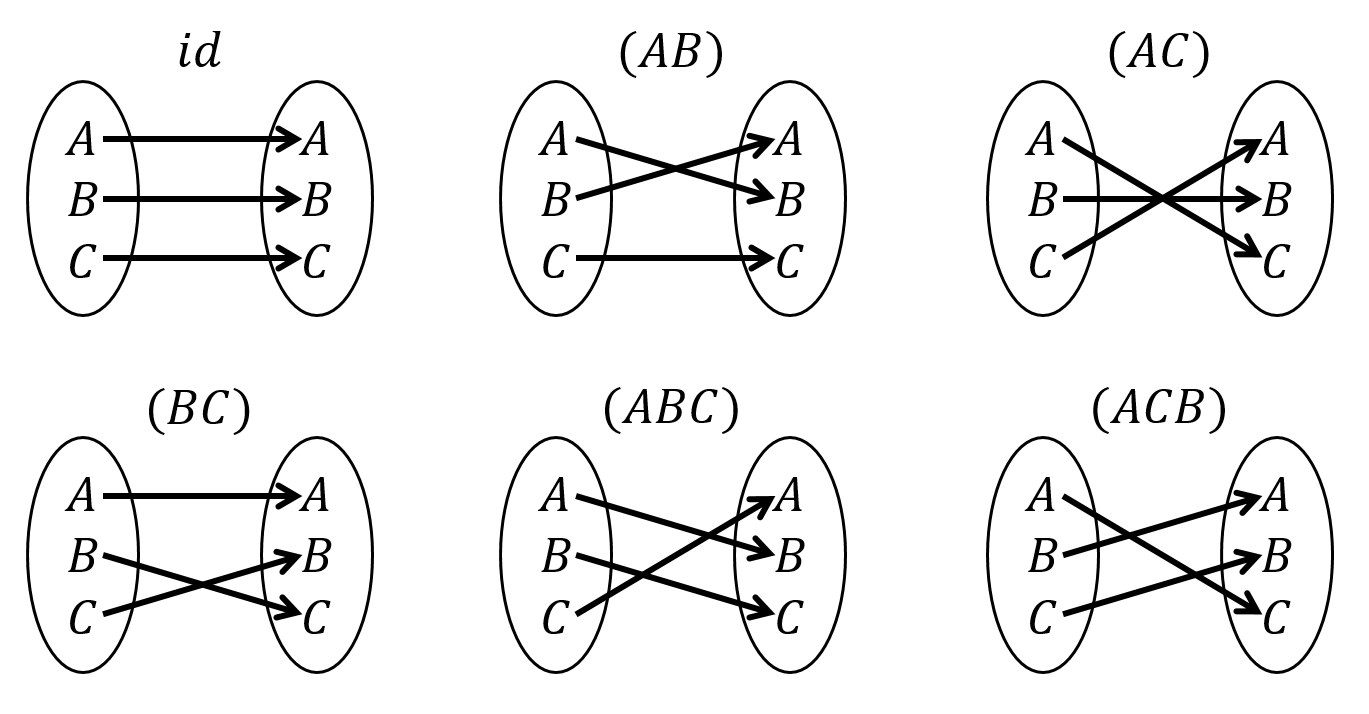
\includegraphics[width=4in]{images/S3onABC.png}
\caption{$S_3$ acting on $X=\{A,B,C\}$.}\label{fig:S3onABC}
\end{center}
\end{figure}

Let's discuss the last element of $S_3$, $(ACB)$. Notice $(ACB)$ ``does something'' to each element of $X$. It maps $A\rightarrow C$, $B\rightarrow A$, and $C\rightarrow B$, so the map images are also elements of $X$. The same is true for all other elements of $S_3$. In fact, each element of $S_3$ produces a bijection on the set $X=\{A,B,C\}$. We refer to this as the group $S_3$ \emph{acting on} the set $X$.
\end{example} 

\begin{example}{Actions2} Let $R$ be the group of all rotations around the origin in $\mathbb{R}^2$. Let $r_d\in R$ denote a counterclockwise rotation of $d$ degrees. Also, let $X$ be the set of all lines through the origin, where $x_d$ denote the line which makes an angle of $d$ degrees with the $x$-axis. See Figure~\ref{fig:rotate_line} below.

\begin{figure}[htbp]
\begin{center}
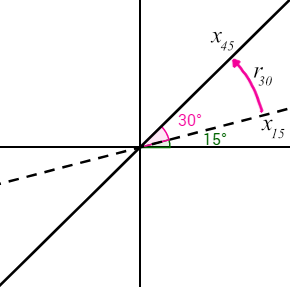
\includegraphics[width=2.5in]{images/rotate_line.png}
\caption{$r_d=r_{30}$ acting on the line $x_d=x_{15}$}\label{fig:rotate_line}
\end{center}
\end{figure}

Note that both $R$ and $X$ are infinite sets (unlike the previous example). As in Example~\ref{example:actions:Actions1}, each element of $R$ ``does something" to each element of $X$. In this case, each element of $R$ rotates an element of $X$, producing another element of $X$. For example, rotating the line $x_{15}$ by $r_{30}$ produces the line $x_{45}$. Furthermore $r_{30}$ can rotate every element of $X$ and \emph{only} produces elements of $X$. This is true for all other rotations in $R$: each element of $R$ produces a bijection on the set $X$. We again say that the group $R$ \emph{acts on} the set $X$.
\end {example}

In the previous two examples we have been talking about a group ``action" which is \emph{different} from the group operation.  For example, the group operation in Example~\ref{example:actions:Actions1} is composition of permutations, but the action is a mapping of points in $\{A,B,C\}$. In Example~\ref{example:actions:Actions2} the group operation is composition of rotations, but the action is a mapping of lines. In order to distinguish the two operations, we will use the period (.) to represent group action. For example the rotation illustrated in Figure~\ref{fig:rotate_line} can be expressed mathematically as $r_{30}.x_{15}=x_{45}$.

Since we have two different operations (the group operation and the group action), we should determine how they interact with each other. We know that two group elements, $g_1$ and $g_2$, can produce a third group element via the group operator because of closure, and that group element can act on a set element, $x$. We would represent this symbolically as $(g_1g_2).x$. But could that process be done differently? Yes, in fact one group element, $g_2$, could act on the set element, $x$, then that resulting set element could be acted on by a different group element, $g_1$. Symbolically we would write this as $g_1.(g_2.x)$. It turns out (and we will verify) that these two processes are equal to each other: $(g_1g_2).x=g_1.(g_2.x)$. We refer to this equality as \term{compatibility}\index{Actions!compatibility property of}.

\begin{example}{Compat1} To investigate this idea of compatibility let's compare $[(AB)(ACB)].C$ and $(AB).[(ACB).C]$ where $(AB),(ACB) \in S_3$ and $B \in X=\{A,B,C\}$. Note: square brackets were used to group because permutations use parentheses. Figure~\ref{fig:Compatibility1} below has the work and a visual representation of the work.

\begin{figure}[htbp]
\begin{center}
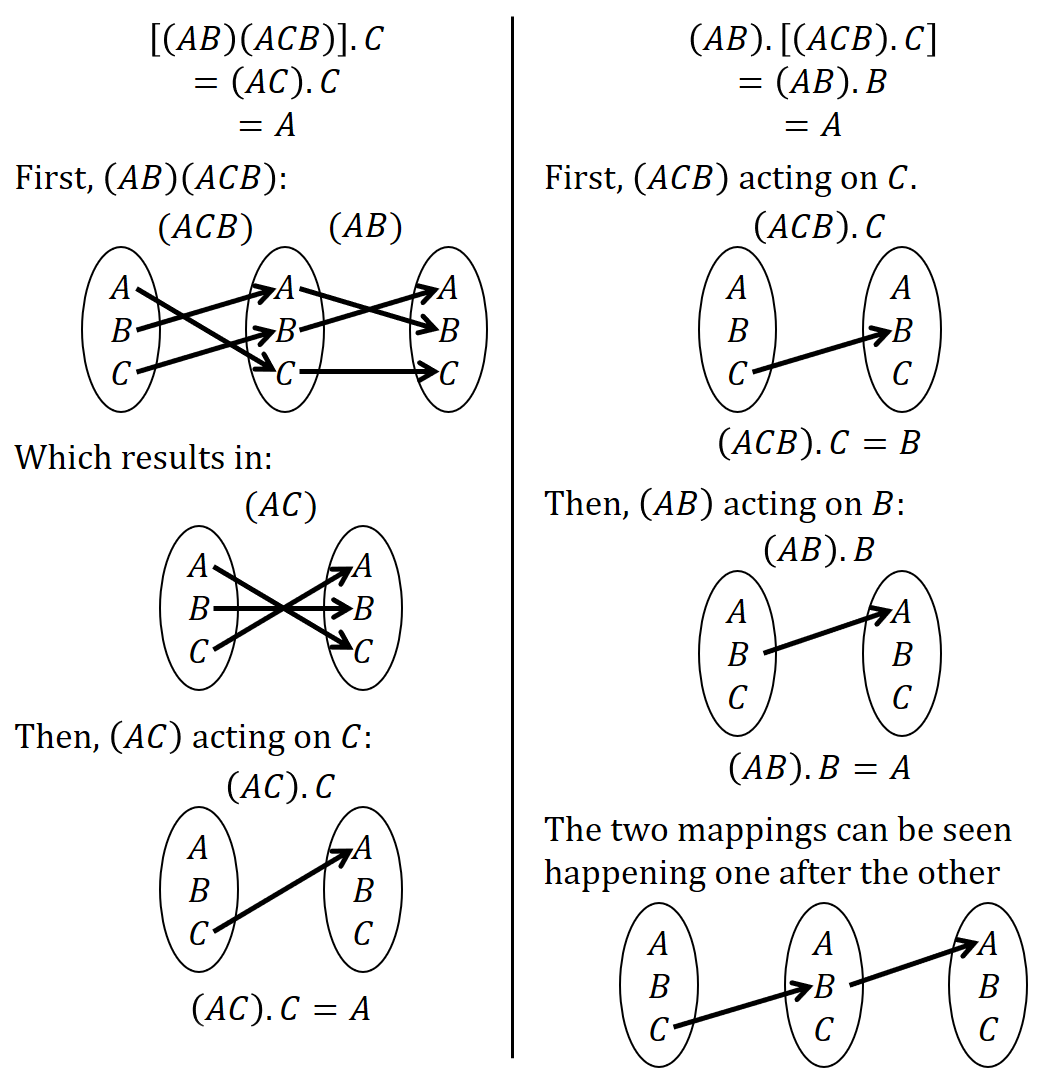
\includegraphics[width=4.75in]{images/Compatibility1.png}
\caption{Formulas and diagrams demonstrating $[(AB)(ACB)].C=(AB).[(ACB).C]$}\label{fig:Compatibility1}
\end{center}
\end{figure}

So, $[(AB)(ACB)].C=A=(AB).[(ACB).C]$, therefore, we can see compatibility in this specific case. Compatibility can be easily shown to hold for the other elements of $X$ because $S_3$ produces a bijection on $X$.

Note the visual difference in the two operations. The group operation of composition of permutations has all the mapping arrows for all elements (the top left two illustrations). This is because the result of a composition of permutations is another permutation. The other illustrations have only one mapping arrow because $S_3$ is acting on $X$ producing only a single element of $X$.
\end {example}

\begin{example}{Compat2} Recall $R$ and $X$ from Example~\ref{example:actions:Actions2}, show that $(r_{40} \circ r_{30}).x_{15}=r_{40}.(r_{30}.x_{15})$.
\begin{equation*}
\begin{split}
(r_{40} \circ r_{30}).x_{15}&\stackrel{?}{=}r_{40}.(r_{30}.x_{15}) \\
 r_{70}.x_{15}&\stackrel{?}{=}r_{40}.x_{45}\\
x_{85}&\stackrel{\checkmark}{=}x_{85}
\end{split}
\end{equation*}
\end {example}

\begin{exercise}{Compat3} Let $G$ be a group acting on the set $X$, and $\sigma, \tau \in G$ and $x \in X$. Using these elements, write a general rule for compatibility between $G$ and $X$.
\end{exercise}

These ideas motivate the following definitions of action and $G$-Set:

\begin{defn}\label{def:action}
Let $G$ be a group and $X$ be a set. A \term{(left) action}\index{Actions!group} of $G$ on $X$ is a map $G\times X\rightarrow X$ given by $(g, x)\rightarrow g.x$, such that
\begin{enumerate}[(1)]
\item Identity: $e.x = x$ for all $x\in X$, and $e$ is the identity element of the group $G$;
\item Compatibility: $(g_1g_2).x = g_1.(g_2.x)$ for all $x\in X$ and all $g_1, g_2 \in G$.
\end{enumerate}
We will use the period to represent group action. The set $X$ on which $G$ acts is called a \term{$G$-set} \index{G-set@$G$-set}.
\end{defn}

\begin{rem}
\begin{enumerate}[(1)]
\item $X$ is not required to be a group, it only needs to be a set. $G$ is the group. In some cases, as we will see, $X$ can be a group.
\item $g.x$ is not group multiplication. It is the result when $g$ acts on $x$, and is always an element of $X$.
\item We call the set $X$ a $G$-set because $G$ is acting on it. If $\mathbb{R}^2$ is acting on $X$ we will call $X$ an $\mathbb{R}^2$-set; $GL_2 (\mathbb{R})$ acting on $X$ would be a $GL_2 (\mathbb{R})$-set.
\item Notice that the second condition in Definition~\ref{def:action} is NOT associativity. It is not associativity because the group operation between $g_1$ and $g_2$ is not the action between $g$ and $x$. Recall we refer to this property as compatibility.
\end{enumerate}
\end{rem}

It is also possible to define right group actions.

\begin{exercise}{RightAction}
Fill in the blanks with the missing information for the definition of right action. Let $G$ be a group and $X$ be a set. A \term{(right) action}\index{Actions!group} of $G$ on $X$ is a map $\underline{~<1>~}\times \underline{~<2>~}\rightarrow \underline{~<3>~}$ given by $(\underline{~<4>~}, \underline{~<5>~})\rightarrow \underline{~<6>~}$, such that
\begin{enumerate}[(1)]
\item Identity: $\underline{~<7>~}=\underline{~<8>~}$ for all $x\in X$, and $e$ is the identity element of the group $G$;
\item Compatibility: $\underline{~<9>~}=\underline{~<10>~}$ for all $x\in X$ and all $g_1, g_2 \in G$.
\end{enumerate}
\end{exercise}

Moving forward in this chapter we'll focus just on left group actions.\index{Actions!left and right}  Following are some more examples of group actions.

\begin{example}{Action3}
Consider $GL_2(\mathbb{R})$ (the group of invertible $2 \times 2$ matrices) and $\mathbb{R}^2$. Show that $GL_2(\mathbb{R})$ acts on $\mathbb{R}^2$ by left multiplication on vectors which means that $\mathbb{R}^2$ is a $GL_2(\mathbb{R})$-set. To check we must show identity and compatibility:
\begin{enumerate}[(1)]
\item Check identity: If $v\in \mathbb{R}^2$ and $I$ is the identity matrix, then $I.v = v$. 
\item Check compatibility: If $A$ and $B$ are $2 \times 2$ invertible matrices, then $(AB).v = A.(B.v)$ since matrix multiplication is associative (see exercise below). Using the associative property is okay here because $\mathbb{R}^2$ vectors can be written as a $2 \times 1$ matrix, so the group operation and the group action are both cases of matrix multiplication. 
\end{enumerate}
Therefore, by definition, $\mathbb{R}^2$ is a $GL_2(\mathbb{R})$-set.
\end{example}

\begin{exercise}{Action4}
Let
\begin{equation*}
A=\left[\begin{array}{cc}
a&b\\c&d\end{array}\right]; \quad 
B=\left[\begin{array}{cc} e& f\\ g & h\end{array}\right]; \quad 
v=\left[\begin{array}{c}x\\ y\end{array}\right].
\end{equation*}
Verify the previous example by showing the associative property of matrix and vector multiplication. 
\end {exercise}

\begin{example}{Action6}
Let $G$ be a group and $\mathcal{E}_n$ be the set of all subsets of $G$ with $n$ elements where $n$ is a positive integer and $n\leq |G|$. Let $S \in \mathcal{E}_n$, meaning $S$ is a subset of $G$ with $n$ elements. Then $G$ acts on $\mathcal{E}_n$ by $g.S:=\{gs~|~s \in S\}$. Note that $g.S$ is a subset of $G$ with $n$ elements. Let's verify that this is an action:
\begin{enumerate}[(1)]
\item Check the identity condition: $e.S=\{es~|~s \in S\}=S$
\item Check the compatibility condition: Let $g,h \in G$, then $(gh).S=\{(gh)s~|~s \in S\}=\{g(hs)~|~s \in S\}=g.(h.S)$
\end{enumerate}
Parts (1) and (2) verify that $\mathcal{E}_n$ is a $G$-set.
\end{example}

To show that $(G,X)$ is \emph{not} an action (in other words $X$ is not a $G$-set), one may show any one of the following:
\begin{itemize}
\item $g.x \notin X$ for some $g \in G$ and $x \in X$;
\item the identity condition fails $e.x \neq x$ for some $x\in X$; or
\item the compatibility condition fails: $(g_1g_2).x \neq g_1.(g_2.x)$ for some $x\in X$ and some $g_1, g_2 \in G$.
\end{itemize}
Usually the easiest way to show one of the above items is by a counterexample.

\begin{exercise}{Action7}
\begin{enumerate}[(a)]
\item 
Let $G = 2\mathbb{Z}$ and let $X =\mathbb{Z}$. Show that $X$ is a $G$-set.
\item Let $X = 2\mathbb{Z}$. Show that $X$ is \emph{not} a $\mathbb{Z}$-set.
\hyperref[sec:actions:hints]{(*Hint*)}
\item Let $G = H_6$ (the complex $6$-th roots of unity (see Section~\ref{sec:RootsOfUnity} in Chapter~\ref{complex}) and let $X =\mathbb{C}$. Show that $X$ is a $G$-set.
\item Let $X = H_8$.  Is $X$ a $\mathbb{C}$-set? Explain.
\hyperref[sec:actions:hints]{(*Hint*)}
\end{enumerate}
\end{exercise}

%Add two exercises: (1) Let $X$ and $Y$ be sets and  $x \in X$ and $y \in Y$, and given an operation (.); why is $x.y$ NOT considered $x$ acting on $y$. Why must one of these sets be a group? (2) Are actions invertable? (bijective map)

\section{Group actions associated with subgroups and cosets}\label{SubgroupsAndCosets}
It turns out that if the set $X$ is also a group, then it's always possible to define a group action of $X$ on itself, where the group action is identical to the group operation: $g.x:=gx$.

\begin{example}{SubgroupAction1}
Consider the group $\mathbb{Z}_5$ which as we know is a group under addition. We will show that $\mathbb{Z}_5$ is a $\mathbb{Z}_5$-set where the group action is $g.x := g+x$. To do this we must show the identity and compatibility conditions. First, $0.x = 0+x = x$ for all $x \in\mathbb {Z}_5$, so the identity condition is met.  Secondly, we need to show compatibility: by the associative property of addition in $\mathbb {Z}_5$, we have $(g_1+g_2).x = (g_1+g_2)+x  = g_1+(g_2+x) = g_1.(g_2.x)$ for all $x, g_1,g_2 \in\mathbb{ Z}_5$. So the compatibility condition is met.  Therefore, by definition of $G$-set, $\mathbb{Z}_5$ is a $\mathbb{Z}_5$-set.
\end {example}

\begin{exercise}{SubgroupAction2}
\begin{enumerate} [(a)]
\item Recall $\mathbb{ Q}^* $ is the nonzero rational numbers under multiplication. Show that $\mathbb{ Q}^* $ is a $\mathbb{ Q}^* $-set.
\item Recall $H_5$ is the complex 5th roots of unity under complex multiplication (see Section~\ref{sec:RootsOfUnity}). Show that $H_5$ is an $H_5$-set.
\item Let $T$ be the unit circle in the complex numbers under multiplication (see Figure~\ref{rtsunity} in Section~\ref{sec:RootsOfUnity}).  Find a group $G$ such that $T$ is a $G$-set, and prove the statement.
\end{enumerate}
\end {exercise}
We can generalize the results of the preceding exercise in the following proposition:

\begin{prop}{GSetSelf} 
For any group $G$, $G$ is a $G$-set with action equal to the group operation in $G$: $g.h:=gh$ for any $g,h \in G$.
\end{prop}

\begin{exercise}{GSetSelf2}: 
Prove the above proposition.
\end {exercise}

\begin{exercise}{SubgroupAction3}
\begin{enumerate} [(a)]
\item Let $G=\{2^n~|~n \in \mathbb{Z}\}$: $G$ is a multiplicative subgroup of $\mathbb{Q}^*$. Show that $\mathbb{Q}^*$ is a $G$-set.
\item Let $T$ be the unit circle in the complex numbers under multiplication.  Show $T$ is an $H_5$-set.
\end{enumerate}
\end {exercise}

In Exercises~\ref{exercise:actions:Action7} and \ref{exercise:actions:SubgroupAction3}, we've seen cases where $G$ is a group and $H$ is a subgroup of $G$.  In this situation, $H$ will always produce a group action on $G$:

\begin{prop}{HSet} 
If $G$ is a group, and $H$ is a subgroup of $G$, then $G$ is an $H$-set using the definition $h.g:=hg$.
\end{prop}

\begin{exercise}{HSet2} 
Prove the above proposition.
\end {exercise}

Recall our discussion of cosets in Chapter~\ref{cosets} In particular, a left coset consists of a group element $g$ acting on a subgroup $H$ of $G$. The group element acts on each element of the subgroup to create a coset. In other words, a coset is a subgroup shifted by action of a group element.  If $G$ is a group, we can let $L$ be the set of left cosets. We will see in the following examples that we can define a group action on $L$.  That is the set of left cosets, $L$ is a $G$-set.
Let $G$ be the additive group of real numbers.  That is, $G=(\mathbb{R},+)$, and let $H$ be all integer multiples of $2\pi$.   That is, $H=\{2k\pi:k\in \mathbb{Z}\}$, or $H = 2 \pi \mathbb{Z}$ for short.  

\begin{exercise}{AngleCoset1}
Prove that $2 \pi \mathbb{Z}$ is a subgroup of $(\mathbb{R},+)$.
\end{exercise}
\begin{example}{AngleCoset2}
Let $L$ be the set of left cosets of $2\pi \mathbb{Z}$ in the group $(\mathbb{R},+)$.  Recall from Definition~\ref{def_coset} in Chapter~\ref{cosets} that the set of left cosets $L$ is defined as $x+2\pi \mathbb{Z}=\{x+h:h\in 2\pi\mathbb{Z}\}$.  For example, the left coset which contains $\pi/3$ is the set $ \{\pi/3 +2k\pi, k\in \mathbb{Z}\}$, which we could also write as $\{ \ldots \pi/3-4\pi, \pi/3-2\pi, \pi/3, \pi/3+2\pi, \pi/3 + 4\pi, \ldots \}$.  It turns out that $L$ is $G$-set under the action  
$(g,x+2\pi\mathbb{Z}) \rightarrow g+x+2\pi\mathbb{Z}$. Let's verify the two conditions of a $G$-set:
\begin{enumerate}[(a)]
\item
For the identity condition note that $e\in G=0$. Then, $0+x+2\pi\mathbb{Z}=x+2\pi\mathbb{Z}$ for any $x+2\pi\mathbb{Z}\in L$.  So the identity condition is true.
\item 
For the compatibility condition consider two real numbers $a,b$.  Then, by associativity of real number addition, $(a+b)+x+2\pi\mathbb{Z}=a+(b+x+2\pi\mathbb{Z})$ for any $x+2\pi\mathbb{Z}$  in $L$.  So the compatibility condition is true.  $L$ is a $G$-set of the additive group of real numbers.
\end {enumerate}
This example has a very practical significance. We know that angles on a unit circle are arbitrary up to multiples of $2\pi$. So we can think of each angle as a coset:  that is, the angle $\theta$ where $0\leq\theta<2\pi$ corresponds to  the coset $\theta + 2\pi \mathbb{Z}$, which represents the set of values $\{\theta +2k\pi\}$, where $k \in \mathbb{Z}$. Now consider what an arbitrary rotation $\phi$ does to the angle $\theta$. For instance, consider the case where $\theta=\frac{\pi}{4}$~--~then $\theta+H=\{ \frac{\pi}{4}+2k\pi\}$.  We'll suppose that the rotation angle is $\phi=\frac{15\pi}{2}$.  According to the group action, $\phi+\theta+H =\frac{15\pi}{2}+\{\frac{\pi}{4}+2k\pi\}$ which will result in the new coset $\{\frac{31\pi}{4}+2k\pi\}=\{\frac{7\pi}{4}+2k\pi\}$.
As we can see, the action of the additive group $(R,+)$ on the cosets $\theta + 2\pi \mathbb{Z}$ corresponds to rotation by arbitrary angles around the unit circle. If the rotation is more than $2 \pi$, the action still works because the cosets take care of any extra factors of $2 \pi$.
\end {example}

In the following exercise you will generalize the above example by showing how the set of all left cosets from a particular subgroup of group $G$ is a $G$-set.

\begin{exercise}{Action5}
Let $G$ be a group and $H$ be a subgroup of $G$. Let $L=\{xH~|~x\in G \}$ which is the set of all left cosets of $H$ in $G$. Then $G$ acts on $L$ by $g.xH = (gx)H$, which is also a coset of $H$. Show that $G$ is acting on $L$, which means that $L$ is a $G$-set.
\end{exercise}

Let's consider another example of group action on a set of cosets.  This example can be thought of as a two-dimensional version of Example~\ref{example:actions:AngleCoset2}, and can be envisioned using computer graphics.

\subsection{The integer lattice}\label{subsec:lattice}

Let $G$ be the $xy$-plane under addition (that is, $G=(\mathbb {R}^2,+)$).  Let $H=\mathbb{Z}\times \mathbb{Z}$, which is a subgroup of $G$ ($H$ is called the \term{integer lattice}\index{Integer lattice}: see Figure~\ref{fig:HwithUnitSquare}).
Cosets of $H$ in $G$ may be written as $a+H=\{(x+m, y+n):m,n \in\mathbb{ Z}\}$, where $a :=(x,y)$ can be any element of $G$. Recall from Proposition~\ref{cosets_theorem_2} that cosets form a partition, so $H$ and its cosets partition $\mathbb{R}^2$.

\begin{figure}[htpb]
\begin{center}
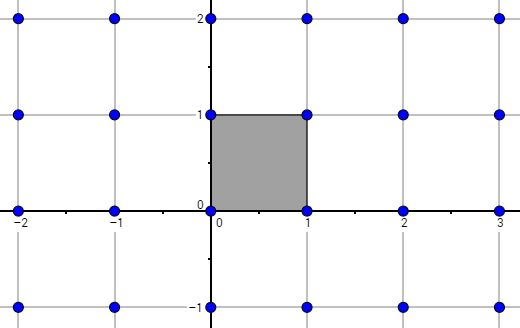
\includegraphics[width=4in]{images/Lattice_Hwithunitsquare.png}
\caption{\label{fig:HwithUnitSquare}Diagram showing $H$ (the integer lattice) with the unit square shaded. This figure and the similar figures in the section were created using the software ``GeoGebra'' (see \url{www.geogebra.org}).  }
\end{center}
\end{figure}

The \term{unit square}\index{Unit square} (the shaded area in Figure~\ref{fig:HwithUnitSquare}) is the area on the $xy$-plane that is $[0,1) \times [0,1)$, meaning the square includes the points on the $x$ and $y$ axes, but not on the lines $x=1$ and $y=1$. Note that $H$ has only one point in the unit square, namely $(0,0)$, similarly any coset of the form $a+H$ has only one point in the unit square (we will prove this mathematically later). We can say that $a\in \mathbb{R}^2$ maps $H$ to produce a coset $a+H$.

\begin{example}{IntLatIntro} Consider a particular group element $a=(0.7,0.5)$. Let's use a graphical illustration to model the point $a$ mapping the integer lattice $H$ which results in the coset $a+H$.

\begin{figure}[htpb]
\begin{center}
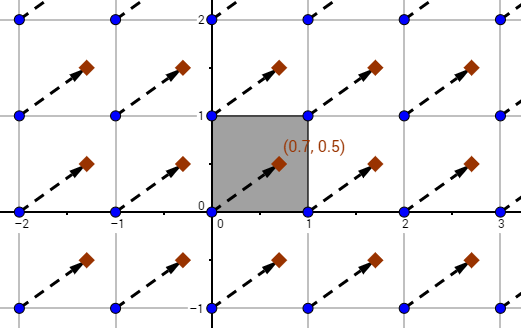
\includegraphics[width=4in]{images/Lattice_xPlusH.png}
\caption{\label{fig:Lattice_xPlusH}The integer lattice, $H$, is represented by blue points, while the elements of the coset $(0.7,0.5)+H$ are represented by red diamonds. The dotted black arrows show the creation of the coset.}
\end{center}
\end{figure}

You can duplicate the above illustration by physically by drawing the coset points (red diamonds) on a plastic transparency, placing it over a graph of the integer lattice (blue points) and moving the transparency $0.7$ units to the right and $0.5$ units upwards.
\end{example}

We will be needing to use the \term{floor function}\index{Floor function}, also known as the greatest integer function. The floor function takes a real number, $x \in \mathbb{R}$ as input and outputs the greatest integer that is less than or equal to $x$. We will use these brackets, $\lfloor~\rfloor$, to represent the floor function. Mathematically we can express this as:
$$\lfloor x \rfloor=\max \{ m\in \mathbb{Z} ~|~m\leq x \}.$$

Here are just a few quick examples: $\lfloor 4 \rfloor = 4$, $\lfloor \pi \rfloor = 3$, and $\lfloor -2.3 \rfloor = -3$.

\begin{exercise}{IntLatBijection} In the following you will show that there is a bijection between cosets of the form $a+H$, where $a\in\mathbb{R}^2$ and points of the unit square.
\begin{enumerate}[(a)]
\item Let $(m,n)$ be the lower left point of the lattice square which contains the point $a$. Using the floor function, give  expressions for $m$ and $n$.
\item Show that $a+(-m,-n)$ is inside the unit square. This implies that $a+H$ contains at least one point inside the unit square.
\item Use proof by contradiction to show that the coset $a+H$ cannot have two different points inside the unit square.
\end{enumerate}
Since each coset $a+H$ contains exactly one point in the unit square, and each point in the unit square is contained in exactly one coset $a+H$, it follows that there exists a one-to-one and onto correspondence (i.e. a bijection) between points in the unit square and cosets of $H$.
\end{exercise}

\begin{example}{IntLat1} Continuing from Example~\ref{example:actions:IntLatIntro}: let $b=(0.8,0.3)$, where $b \in G$. Find the point $h=(m,n) \in H$ such that $b+a+h$ is inside the unit square (recall $a=(0.7,0.5)$).

The element $b$ acts on the coset $a+H$ as follows:  
\begin{align*}
 b+a+H &=\{(0.8+(0.7+m), 0.3+(0.5+n)):m, n \in \mathbb{Z}\}\\
&=\{(0.8+0.7+m, 0.3+0.5+n):m, n \in \mathbb{Z}\}\\
&=\{(1.5+m, 0.8+n):m, n \in \mathbb{Z}\}. 
\end{align*}
If $m=-1$ and $n=0$, then $b+a+h=(1.5-1,0.8+0)=(0.5,0.8)$, so $h=(-1,0)$.
\end{example}

\begin{exercise}{floorh} Generalize the above example as follows. Let $a,b \in \mathbb{R}^2$ such that $a=(a_x,a_y)$ and $b=(b_x,b_y)$. Let $h=(m,n)$ where $m=-\lfloor b_x+a_x \rfloor$ and $n=-\lfloor b_y+a_y \rfloor$ (note that $h \in H$). Verify graphically the formulas for $m$ and $n$, and show algebraically that $b+a+h$ is in the unit square.
\end{exercise}

The point $b+a+h=(0.5,0.8)$ is the \emph{only} point of the coset $b+a+H$ which is inside the unit square. By basic properties of cosets, it follows that $b+a+H =(0.5, 0.8)+H$. Recall that by definition a left coset of the integer lattice $a+H$ means adding the same point, $a=(x,y)$, to each point in the integer lattice, $H$. A group action simply changes one coset of $H$ in $G$ to a different coset.  The top illustration in Figure~\ref{fig:IntegerLattice1} show the displacement of the coset $a+H$ when acted on by $b$ on the left from Example~\ref{example:actions:IntLat1}. 

\begin{figure}[htpb]
\begin{center}
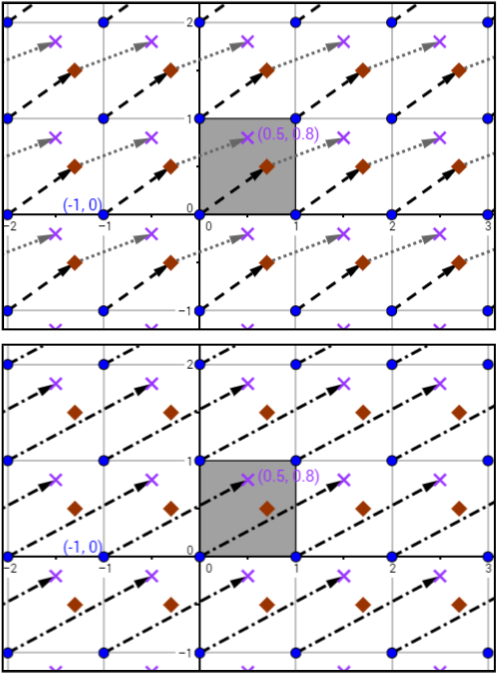
\includegraphics[width=4.0in]{images/Lattice_baHcH.png}
\caption{From Example~\ref{example:actions:IntLat1}, the top figure is illustrating the displacement of the coset $a+H$ for $a=(0.7,0.5)$ when acted on by $b=(0.8,0.3)$ on the left. The bottom figure is illustrating the coset $c'+H$, where $c'=b+a$. The lattice, $H$ is represented by blue points, the elements of the coset $a+H$ are represented by red diamonds, and the elements of the final coset $b+a+H=c'+H$ are represented by purple crosses.}
\label{fig:IntegerLattice1}
\end{center}
\end{figure}

Our above discussion can help us describe the motion of a character on the screen of a ``wraparound'' video game.  Imagine the unit square is your TV or computer screen. Suppose the character starts near the right edge at the point $a=(0.7,0.5)$, and undergoes linear motion to the right and up in the direction of the displacement vector $b=(0.8,0.3)$. Then he moves off the right edge of the screen and re-appears instantly at the left edge, ending up at the previously found point $c=(0.5,0.8)$ as shown in Figure~\ref{fig:wraparound1}. So the point $b+a+h=c$ where $h=(-1,0)$.

\begin{figure}[htpb]
\begin{center}
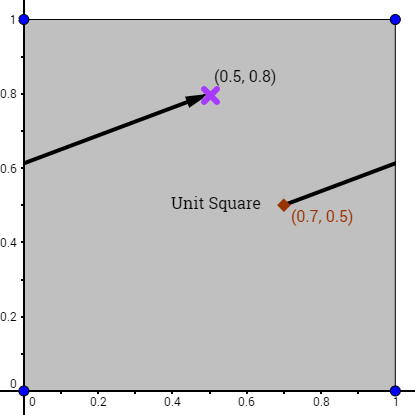
\includegraphics[width=3in]{images/Lattice_wraparound1.png}
\caption{\label{fig:wraparound1}Demonstrating the ``wraparound" effect, when only viewing the unit square, when $b=(0.8,0.3)$ acts on the coset $a+H$ where $a=(0.7,0.5)$.}
\end{center}
\end{figure}

In our conclusion of Exercise~\ref{exercise:actions:IntLatBijection}, we found that there's a bijection between the points of the unit square and the cosets of $H$. So instead of observing an entire coset, we only need to look at the point that is currently inside the unit square, as seen in Figure~\ref{fig:wraparound1} for example. What appears to be a jumpy motion in the unit square (i.e. when the point jumps from the right edge to the left edge) can also be understood in terms of a continuous ``motion" of cosets.

\begin{example}{IntLat2} Consider group elements $a=(-0.6,-0.4)$ and $b=(0.9,1.6)$ where $a,b \in \mathbb{R}^2$.
Let's first find the point $h=(m,n) \in H$ such that $b+a+H$ is inside the unit square. From Exercise~\ref{exercise:actions:floorh}, $m=-\lfloor -0.6+0.9 \rfloor=-\lfloor 0.3 \rfloor=0$ and $n=-\lfloor -0.4+1.6 \rfloor=-\lfloor 1.2 \rfloor=-1$, so $h=(0,-1)$

Next, let's find the point $b+a+h$ in the unit square, let's call this point $c$. $$c=(0.9,1.6)+(-0.6,-0.4)+(0,-1)=(0.3,0.2)$$ So $c=(0.3,0.2)$ and is a point inside the unit square.

Lastly, let's graph the ``movement" of the points that are visible to only the unit square throughout the group action $b$ on $a+H$. Similar to Figure~\ref{fig:wraparound1}.

The Figure~\ref{fig:Lattice2} (top) we have shown ``paths" which follow the action of $b$ on $a+H$. Note that each path is a continuous straight segment. However, if we restrict our field of view to the unit square (see Figure~\ref{fig:Lattice2} (bottom)), there appears to be four disconnected segments, but the top figure shows us how these can be envisioned as a continuous motion.

\begin{figure}[htpb]
\begin{center}
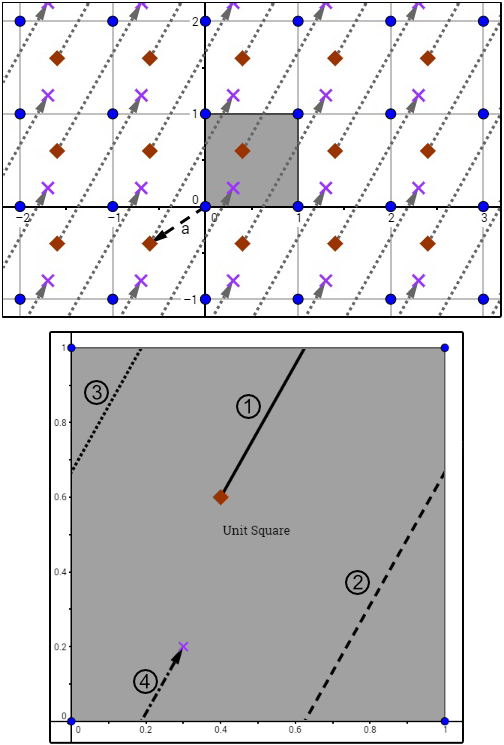
\includegraphics[width=4.0in]{images/Lattice2.png}
\caption{The top figure is illustrating the movement of the coset $a+H$ for $a=(-0.6,-0.4)$ when acted on by $b=(0.9,1.6)$ on the left (only one arrow, labeled $a$, representing the movement of $a$ acting on $H$ is shown so the image wouldn't be cluttered). The bottom figure is illustrating the ``wraparound" effect when only viewing the unit square. The movements are numbered in order and there are different patterns for clarity.}
\label{fig:Lattice2}
\end{center}
\end{figure}

\end{example}

\begin{exercise}{IntLatHW1}
\begin{enumerate}[(a)]
\item Given $a=(0.8,0.6)$ and $b=(1.4,0)$ find the point $h\in H$ such that $b+a+h$ is inside the unit square, and find $c$ in the unit square, such that $c+H=b+a+H$.
\item Given $a=(0.8,0.6)$ and $b=(1.2,1.3)$ find the point $h\in H$ such that $b+a+h$ is an element of the unit square, and find $c$ in the unit square, such that $c+H=b+a+H$.
\item Given $a=(0.8,0.6)$ and $b=(0,3.5)$ find the point $h\in H$ such that $b+a+h$ is inside the unit square, and find $c$ in the unit square, such that $c+H=b+a+H$.
\item Illustrate the first part (a) with a graph.  Graph the point $a+h$.  Then graph the point $b+a+h$, or simply $c$.  Include ordered pairs to indicate the position of these points. Include arrows to indicate the apparent ``movement'' from the point $a+h$ to the point $c$ within the unit square.
\item Create similar graphs illustrating parts (b) and (c).
\end{enumerate}
\end{exercise}

\begin{exercise}{IntLatNotGset} Show that $H$ is \emph{not} an $\mathbb{R}^2$-set. \hyperref[sec:actions:hints]{(*Hint*)}
\end{exercise}

\begin{exercise}{SetOfCosetsGset} Show that the set of all cosets of the form $\{a+H, a \in \mathbb{R}^2\}$ is a $\mathbb{R}^2$-set by answering the following:
\begin{enumerate}[(a)]
\item Let $b \in \mathbb{R}^2$. Define the action of $b$ on $(a+H)$ (in other words complete the following equation: $b.(a+H)=$~?).
\item Prove the identity condition.
\item Prove the compatibility condition.
\end{enumerate}
\end{exercise}


We can think about this example in another way. Suppose we have a \emph{torus}, which is the mathematical word for a donut shape. We could imagine creating a ``map'' of the surface of the torus by cutting the torus apart as shown in Figure~\ref{fig:Torus1}. If we spread this map out flat, it would look like a square (see Figure~\ref{fig:Torus2}). If we wanted to use the map to chart motion on the surface of the torus, then any motion that goes off the right edge would reappear at the left edge; and any motion that goes off the top edge would reappear at the bottom. So you see this is exactly what we saw for the previous example. So using cosets of $\mathbb{Z}^2$ in $\mathbb{R}^2$, we've created a mathematical representation for motion on the surface of a torus.

\begin{figure}[ht]
\begin{center}
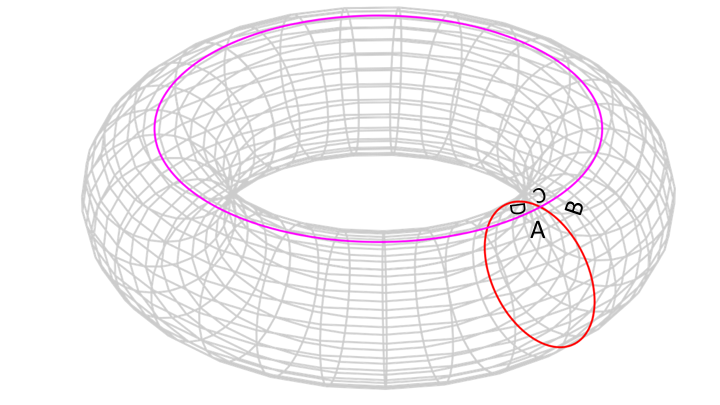
\includegraphics[width=3in]{images/Torus1.png}
\caption{Torus, showing two cut lines.}\label{fig:Torus1}
\end{center}
\end{figure}

\begin{figure}[ht]
\begin{center}
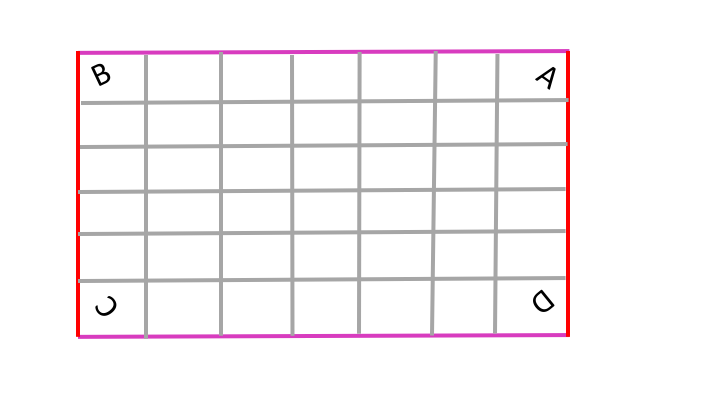
\includegraphics[width=3in]{images/Torus2.png}
\caption{The cut torus, flattened out.}\label{fig:Torus2}
\end{center}
\end{figure}

We can generalize the two previous examples by considering cosets of a subgroup $H$ in a group $G$ that contains $H$.

\begin{example}{CosetAction}
Let $H$ be a subgroup of $G$ and $L_H$ the set of left cosets of $H$. The set $L_H$ is a $G$-set under the action 
$g.(xH)=(gx)H$ (note that $gx\in G$ so $(gx)H$ is a coset of $H$).
Again, it is easy to see that the identity condition is true. Since $(gg').(xH) =(gg'x)H=g.((g'x)H)= g.(g'.(xH))$, the compatibility condition is also true.
\end{example}
So far, we've been looking at group actions on left cosets.  What about right cosets?  Let's investigate.

\begin{exercise}{RtCosetAction}
Consider the case where $G=S_3$, $H=\{\var{id},(12)\}$, and $R$ is the set of right cosets of $H$.  Define a function from $G\times R\rightarrow R$ by $(g,R)\rightarrow Rg$. Does this function define a group action of $G$ on $R$? 
\hyperref[sec:actions:hints]{(*Hint*)}
\end {exercise}
The previous exercise shows that we can't always do the same thing with right cosets that we can do with left cosets.  Let's look at an alternative:  

\begin{exercise}{RtCosetAction2}
\begin{enumerate}[(a)]
\item Repeat the previous exercise, but this time use the function $(g,R)\rightarrow Rg^{-1}$.
\item Show that in general the function $(g,R)\rightarrow Rg^{-1}$ defines an action of $G$ on the right cosets of $H$.  
\end {enumerate}
\end {exercise}

\section{Symmetries of regular polyhedra}\label{ActionsOnPolyhedra}
We want to apply our new ideas to gain insight about the groups of rotational symmetries of \term{regular polyhedra}\index{Polyhedron!regular}  In general, a \emph{polyhedron} can be thought of as a collection of faces, edges and vertices: for example, a cube has 6 faces, 12 edges and 8 vertices. A \emph{regular polyhedron} is a polyhedron in which all faces are congruent regular polygons, and the same number of edges meet at every vertex. The group of rotational symmetries of a polyhedron act on the faces, edges and vertices.  Any rotational symmetry will always take faces to faces, edges to edges and vertices to vertices. 

In the following discussion we'll be introducing a bunch of new ideas. As usual, we'll illustrate these ideas first on a particular example. So let's begin with the cube, which is perhaps the regular polyhedron which is easiest to understand.

\subsection{$G$-equivalence and orbits}
Some of the rotational symmetries of the cube are indicated in Figure~\ref{fig:CubeRot}.
\footnote{Note that these are NOT the only rotational symmetries of the cube--we'll discuss the others later (see  this excellent video: \url{www.youtube.com/watch?v=gBg4-lJ19Gg}).}
The figure shows three possible rotation axes. We will denote the $90^{\circ}$ counterclockwise rotations around the $x,y$ and $z$ axes as $r_x, r_y,r_z$ respectively.  We will also denote the faces of the cube as $x_-, x_+,y_-,y_+,z_-,z_+$.  For example the rotation $r_x\compose r_x=r_x^2$ will take the bottom face ($z_-$) to the top face ($z_+$). 

\begin{figure}[ht]
\begin{center}
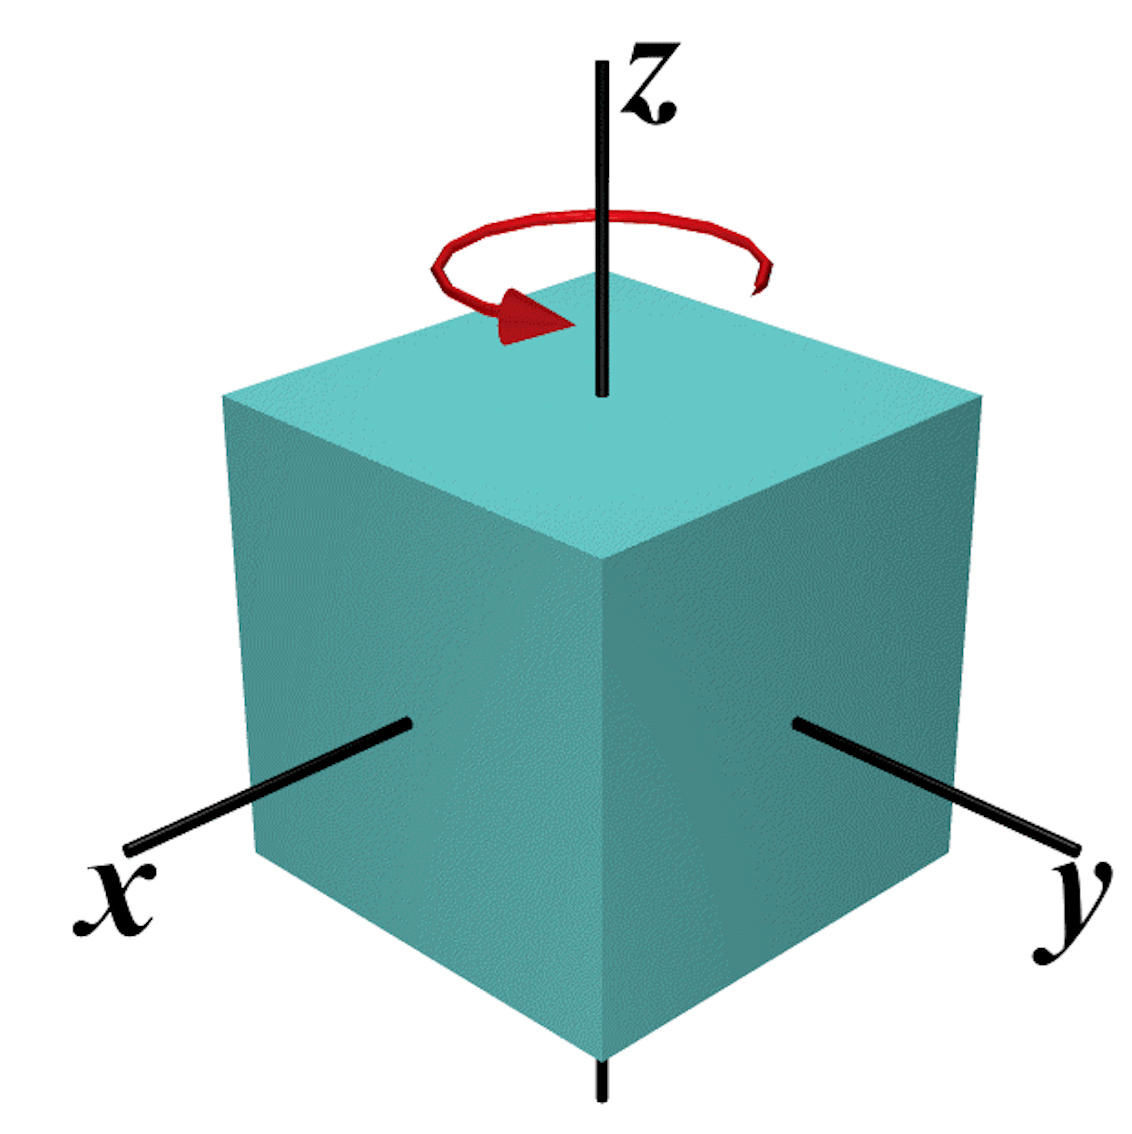
\includegraphics[width=2in]{images/AxesOfCube.png}
\caption{Cube with 3 axes of rotation that give symmetries.}\label{fig:CubeRot}
\end{center}
\end{figure}

\begin{rem} When we rotate the cube, the axes remain \emph{fixed} while the cube rotates around them.  So in Figure~\ref{fig:CubeRot} you may imagine the axes to be like ``laser beams'' going through the cube, where the laser beams are labeled $x, y$ and $z$ according to their axes. These laser beams and labels do not move when the figure is rotated. For example, consider the rotation $r_z$ followed by $r_x$ (which is written as $r_x\circ r_z$). Under $r_z$, the face $x_+$ will rotate where the $y_+$ face was. Then following rotation $r_x$ will occur around the original laser beam $x$ axis, and not the axis to where the $x_+$ face has moved (which would be the rotation $r_y$). The cube ends up with the face $x_+$ on the top with the $z$ axis, $y_+$ on the negative side of the $x$ axis, and $z_+$ on the negative side of the $y$ axis.
\end{rem}

\begin{figure}[ht]
\begin{center}
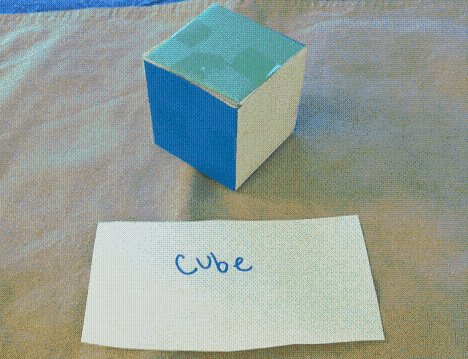
\includegraphics[width=2.5in]{images/CubeFold.png}
\caption[caption]{A paper cube to print, cut and fold 
\\ \hspace{\textwidth} 
(from \url{www.korthalsaltes.com}).}
 \label{fig:CubeFold}
\end{center}
\end{figure}

\begin{rem} Make or find a physical manipulative of a cube. This can be a 6-sided die or constructed from paper as seen in Figure~\ref{fig:CubeFold}. When working with a manipulative of your polyhedron it is a good idea label each face uniquely, whether by color, letter, number, or symbol. If you label your faces $x_+, x_-, y_+,$ etc., make sure to remember that these refer to \emph{faces} and not \emph{axes} (as we said above, the axes are like fixed laser beams that don't move with the cube).  It also helps to take a picture or two of your manipulative when in its starting position. You might also draw a pair of $x$ and $y$ axes on a spare sheet of paper, set this on the table, and rotate your cube above this paper.
\end{rem}

\begin{exercise}{Cube1}
\begin{enumerate}[(a)]
\item Give rotations that take the bottom face ($z_-$) to each of the faces $x_-,x_+,y_-,y_+$.
%$r_y$ or $r_y^{-3}$takes $z_-\rightarrow x_-$, $r_y\compose r_z^2$ or  $r_y^{-1}$ or $r_y^3$ takes $z_-\rightarrow x_+$, $r_x^3$ or $r_x^{-1}$takes $Z_-\rightarrow y_-$, r_x$ or $r_x^{-3}$takes $z_-\rightarrow y_+$,
\item Give rotations that take the face $y_- $ to each of the faces $x_-,x_+,y_+,z_-,z_+$.
%$r_z^{-1}$or $r_x^{3}$ takes $y_-\rightarrow x_-$, $r_z$ or $r_z^{-3}$ takes %$y_-\rightarrow x_+$, $r_z^{-2}$ or $r_z^{2}$takes $y_-\rightarrow y_+$, $r_x$ %or r_x^{-3} takes $y_-\rightarrow z_-$, $r_x^{-1}$or $r_x^{3}$ takes $y_-\rightarrow z_+$,
\item Let's define a notation for the cube's vertices as follows.  For example, $+++$ represents the vertex in the first octant ($x>0,y>0,z>0$).  The vertex $+-\,-$ will be in the octant where $x>0,y<0,z<0$ (Which is the vertex at lower left in Figure~\ref{fig:CubeRot}).  Give rotations that take the vertex $+-\,-$ to each of the of the vertices 
\[ +++, ~-\,++,~+\,-\,+,~ ++\,-,~-\,-\,+,~-\,+\,-,~-\,-\,-. \]
%$r_x^2$or $r_x^{-2}$ takes $+-\,-\rightarrow +++$,
 %$r_x$ or$r_x^{-3}$ takes $+-\,-\rightarrow -\,++$, 
%$r_x\compose r_y^2$ takes $+-\,-\rightarrow -\,++$, 

\item Let's denote the edges of the cube as follows.  For example, $\overline{x_+z_-}$ represents the edge where the faces $x_+$ and $z_-$ meet.  The edge $\overline{x_+y_-}$ is where the faces $x_+$ and $y_-$ meet.  (This is the left, front-facing edge of cube in Figure~\ref{fig:CubeRot}.)  
\begin{enumerate}[(i)]
\item Using the above notation, list all edges of the cube.
\item Give rotations that take the edge $\overline{x_+y_+}$ to each of the other edges. 
\end {enumerate}
\end{enumerate}
\end{exercise} 
%$\overline{x_+y_-}$, $\overline{x_+z_+}$,$\overline{x_+z_-}$,$\overline{x_-%y_+}$,$\overline{x_-y_-}$,$\overline{x_-z_+}$,$\overline{x_-z_-%}$,$\overline{y_+z_+}$,$\overline{y_+z_-}$,$\overline{y_-z_+}$,$\overline{y_-z_-}$,
%In part (a) of the previous exercise, we saw that we could rotate the bottom face of the cube ($z_-$) to any other face.  We can use this information to rotate between any two faces.  For example, if we want to rotate the top face ($z_+$) to $x_+$, we can do this in two stages as follows.  First, we can rotate $z_+$ to $z_-$ using $r_x^{-1}\compose r_x^{-1}$ (which is the \emph{inverse} of the rotation that we used to take $z_-$ to $z_+$).  Second, we follow this by a rotation that takes $z_-$ to $x_+$ (such as $r_y^{-1}$).  In summary, we then have that 
From the previous exercise it's pretty clear that for any two faces of a cube there is at least one symmetry that takes the first face to the second.  In other words, if $A$ and $B$ represent faces then there always exists a symmetry $g$ such that $gA=B$.  This example motivates the following definition.

\begin{defn}\label{GEquivalent}
If a group $G$ acts on a set $X$ and $x, y \in X$, then $x$ is said to be
\term{$G$-equivalent}\index{G-equiv@$G$-equivalent} to $y$ if there exists a
$g \in G$ such that $gx =y$. We write $x \sim_Gy$ or $x \sim y$ if
two elements are $G$-equivalent.
\end{defn}
By this definition we can say that all faces of a cube are $G$-equivalent to each other under the group of rotational symmetries of a cube, because given any two faces we can always find a rotation that takes the first face to the second face (and the inverse rotationtakes the second face back to the first face).
The notation we're using strongly suggests that $\sim_G$ must be an equivalence relation.  If fact this is true:

\begin{prop}{}
Let $X$ be a $G$-set. Then $G$-equivalence is an equivalence relation
on $X$. 
\end{prop}
\begin{proof}
The relation $\sim$ is reflexive since $ex = x$. Suppose that $x \sim
y$ for $x, y \in X$. Then there exists a $g$ such that $gx = y$. In
this case $g^{-1}y=x$; hence, $y \sim x$. To show that the relation is
transitive, suppose that $x \sim y$ and $y \sim z$. Then, there must
exist group elements $g$ and $h$ such that $gx = y$ and $hy= z$. So $z
= hy = (hg)x$, and $x$ is equivalent to $z$.
\end{proof}

Recall from Chapter~\ref{EquivalenceRelationsChap} that every equivalence relation on a set $X$ is associated with a partition of $X$, where a partition is a collection of disjoint subsets whose union is $X$. Each set in this partition is called an \term{equivalence class}.\index{Equivalence class}

\begin{exercise}{Cube2}
Consider the edge $\overline{y_+z_+}$ of a cube.  What is the equivalence class of this edge under $G$-equivalence, where $G$ is the group of rotational symmetries of a cube? \emph{Explain} your answer.
\end {exercise}

In the case of a cube where $X=\{\text{faces}\}\cup\{\text{edges}\}\cup\{\text{vertices}\}$ The three sets $\{\text{faces}\},\{\text{edges}\},\{\text{vertices}\}$ are disjoint equivalence classes whose union is $X$. We call each of these sets an \emph{orbit} of $X$ under $G$.  In general, we have the following definition.

\begin{defn} \label{noteorbit}
If $X$ is a $G$-set, then each set in the partition of $X$ associated with
$G$-equivalence is called an \term{orbit}\index{Orbit!Of a $G$-set} of $X$ under $G$. We will denote the orbit that contains an element $x$ of $X$ by
${\cal O}_x$. 
\end {defn}
The next example shows how these concepts apply to permutation groups as well.

\begin{example}{Orbit1}
Let $G$ be the permutation group defined by
\[
G =\{(1), (1 23), (1 3 2), (4 5), (1 2 3)(4 5), (1 3 2)(4 5) \}
\]
and $X = \{ 1, 2, 3, 4, 5\}$. Then $X$ is a $G$-set. There are permutations in $G$ that take $1\rightarrow2$, $1\rightarrow3$, $2\rightarrow3$, and vice versa. There are also permutations that take $4\rightarrow 5$ and vice versa.  So the orbits are $\{1, 2, 3\}$ and $\{4, 5\}$. 
\end{example} 
 
\begin{exercise}{orbits2}
\begin{enumerate}[(a)]
\item Let $G=\{\var{id},\mu_1\}$ which is a subgroup of $S_3$ (the symmetry group of an equilateral triangle) (See Figure~\ref{groups_s3_symmetry_fig} in Section~\ref{SymmetryGroup}.) Let $X=\{A,B,C\}$ be the set of vertices of an equilateral triangle. List the orbits of $X$ under $G$
\item Let $G$ be the permutation group defined by
\begin{align*}
G =&\{(1), (1358),(15)(38), (1853), (247),(274), (1358)(247),(15)(38)(247),\\
&~~ (1853)(247),(1358)(274),(15)(38)(274),(1853)(274) \}
\end{align*}
and $X = \{ 1, 2, 3, 4, 5,6,7,8\}$. Then $X$ is a $G$-set.  List the orbits of $X$ under $G$.
\end{enumerate}
\end {exercise}


\subsection{Stabilizers, stabilizer subgroups, and fixed point sets}

 Let's return to the cube to illustrate another new concept. Every rotation of a cube has an axis of rotation as well as an angle.   
 For rotations which are symmetries we've considered 3 possible axes, passing through opposite pairs of faces. 
Take for instance the axis which passes through $x_+$ and $x_-$, and consider the set of all the rotational symmetries having this axis.
In fact, this set of symmetries forms a subgroup  of the symmetries of the cube (in this case, the subgroup is isomorphic to the rotations of the square or ($\integer_4$,+)). Now all of the elements of this subgroup leave the face  $x_+$ fixed (although $x_+$ rotates, it remains in the same place).
Similarly, the rotations about the axis through $y_+$ and $y_-$ form a subgroup whose elements leave  $y_+$ fixed; and the rotations about the axis through $z_+$ and $z_-$ behave the same way for $z_+$.  

 These are all examples of \emph{stabilizer subgroups}. The general definition is as follows.

\begin{defn}\label{StabilizerSubgroups} 
Given that $X$ is a $G$-set and  $x \in X$, let $G_x$ be the set of  group elements $g$ that fix $x$:  in other words, $gx=x$.  Then $G_x$ is called the \term{stabilizer subgroup}\index{Subgroup!stabilizer} or \term{isotropy 
subgroup}\index{Subgroup!isotropy} of $x$.
\end{defn}

The above definition presumes that $G_x$ is in fact a subgroup, which up until now we haven't proved. The following exercise remedies this deficiency:

\begin{exercise}{Stabilizer1}
Given any $x$ in $X$, prove that the stabilizer subgroup $G_x$  is indeed a subgroup of $G$.  (Recall this involves proving closure under composition and inverse.)
\end {exercise}

Definition~\ref{StabilizerSubgroups} talks about elements of the group $G$ which leave a particular element of set $X$ fixed. We can turn this around and consider elements of $X$ which are fixed by a particular element of $G$. In fact, each element of $G$ has an associated subset of $X$ that it leaves unchanged. 

Consider for instance the group of rotations of a cube. We may describe the cube as consisting of faces, edges, and vertices. So let's take   $X=\{\text{faces}\}\cup\{\text{edges}\}\cup\{\text{vertices}\}$.  Rotations about the $x$ axis (which can all be expressed as ${r_x}^n$ for some $n$) leave the faces $x_+$ and $x_-$ fixed. Similarly, $\{y_+$ ,$y_-\}$ and $\{z_+,z_-\}$ are  fixed by rotations about the $y$ axis and $z$ axis, respectively.   Thus, $\{x_+,x_-\},\{y_+,y_-\},\{z_+,z_-\},$  are all examples of \emph{fixed point sets} in $X$.
This leads to another definition:

\begin{defn} \label{FixedPoint}
Let $G$ be a group acting on a set $X$, and let $g$ be
an element of $G$. The \term{fixed point set}\index{Fixed point
set!of a group element} of $g$ in $X$, denoted by $X_g$, is the set of 
all $x \in X$ such that $gx = x$.
\end{defn}
\noindent
It is important to remember that $X_g \subset X$ and $G_x \subset G$. 

Let's use this notation to describe some stabilizer subgroups and fixed point sets for familiar examples of group actions.

\begin{example}{FixedPoint1}
Let $G$ be the rotational symmetries of a cube and $X=\{\text{faces}\}\cup\{\text{edges}\}\cup\{\text{vertices}\}$.
The fixed point set of $\var{id}$ is: 

$$X_{\var{id}}=\{\text{faces}\}\cup\{\text{edges}\}\cup\{\text{vertices}\},$$
since the identity rotation  leaves the entire cube unchanged.  
\end {example}

\begin{example}{FixedPoint2}
Let's consider the stabilizer subgroups for the faces of a cube.  These contain the elements of the group $G$ of rotations of the cube that leave each face unchanged.  The stabilizer subgroups for the faces are:
$$\begin{array} {c}
G_{x_+}=G_{x_-}=\{\var{id},r_x,r_x^2,r_x^3\}\\
G_{y_+}=G_{y_-}=\{\var{id},r_y,r_y^2,r_y^3\}\\
G_{z_+}=G_{z_-}=\{\var{id},r_x,r_x^2,r_x^3\}
\end {array}$$
\end{example}

\begin{example}{FixedPoint3}
Let $X = \{1, 2, 3, 4, 5, 6\}$ and suppose that $G$ is the permutation
group given by the permutations 
$$\{(1), (1 2)(3 4 5 6), (3 5)(4 6), (1 2)( 3 6 5 4)\}.$$
Then the fixed point sets of $X$ under the action of $G$ for the different group elements are
$$
\begin{array}{c}
X_{(1)} = X, \\
X_{(3 5)(4 6)} = \{1,2\}, \\
X_{(1 2)(3 4 5 6)} = X_{(1 2)(3 6 5 4)} = \emptyset,
\end{array}
$$
and the stabilizer subgroups for the different elements of $X$ are
$$
\begin{array}{c}
G_1 = G_2 = \{(1), (3 5)(4 6) \}, \\
G_3 = G_4 = G_5 = G_6 = \{(1)\}.
\end{array}
$$
\end{example}

%\begin{thm}
%Let $G$ be a group acting on a set $X$ and $x \in X$. The stabilizer
%group, $G_x$, of $x$ is a subgroup of $G$. 
%\end{thm}
%\begin{proof}
%Clearly, $e \in G_x$ since the identity fixes every element in the
%set $X$. Let $g, h \in G_x$. Then $gx = x$ and $hx = x$. So $(gh)x =
%g(hx) = gx = x$; hence, the product of two elements in $G_x$ is also
%in $G_x$. Finally, if $g \in G_x$, then $x = ex = (g^{-1}g)x =
%(g^{-1})gx = g^{-1} x$. So $g^{-1}$ is in $G_x$. 
%\end{proof}

\begin{exercise}{}
Let $G = S_4$ (the permutations of 4 elements), and let $X = \{1,2,3,4\}$.  $X$ is a $G$-set.
\begin{enumerate}[(a)]
\item
Give $G_2$, $G_4$, and $G_2 \cap G_4$.  Is $G_2 \cap G_4$ a group? \emph{Explain} your answer.
\item
Give $X_{(123)}$, $X_{(234)}$,and  $X_{(123)} \cap X_{(234)}$.
\item
Repeat part (a) with $G=A_4$ (the group of even permutations on 4 elements).
\item
Repeat part (b) with $G=A_4$ (the group of even permutations on 4 elements).
\end{enumerate}
\end{exercise} 
As usual, we will denote the number of elements in the fixed point set of an
element $g \in G$ by $|X_g|$, the number of elements of the stabilizer subgroup of $x\in X$ as $|G_x|$ and the number of elements in the orbit of $x \in X$ by $|{\cal O}_x|$.

\begin{exercise}{}
Let $G = S_n$ (the permutations of n elements), and let $X = \{1,2,\ldots n \}$.  $X$ is a $G$-set.
\begin{enumerate}[(a)]
\item
What is $|G_1|$? What is $|G_2|$? What is $|G_k|$ where $k \in X$?  (Recall that $|S_n| = n!$)
\item
If $g$ is a $3$-cycle, then what is $|X_g|$? What if $g$  is a 5-cycle?  (You may assume that $n \ge 5$).
\item
Give a general formula for $|X_g|$, where $g$ is a $k$-cycle ($2 \le k \le n$).
\item
Repeat part (a) with $G = A_n$ (the even permutations of $n$ elements).
\item
Repeat part (b) with $G = A_n$.
\item
Repeat part (c) with $G = A_n$.
\end{enumerate}
\end{exercise}

%Recall from Chapter\ref{cosets} that the \emph{index} of $G_x$ in $G$ (denoted by $[G:G_x]$) is the number of cosets of $G_x$. 

\subsection{Counting formula for the order of  polyhedral rotational symmetry groups}

It is possible to characterize the size of the rotational symmetry group $G$ for a regular polyhedron in terms of $|{\cal O}_x|$and $|G_x|$. We'll show this with an example.

\begin{example}{CountingFormula1} 
Consider our old friend the group of rotational symmetries of a cube acting on $X=\{\text{faces}\}\cup\{\text{edges}\}\cup\{\text{vertices}\}$. We've seen that $G_{x_+}=\{\var{id},r_x,r_x^2,r_x^3\}$ is the stabilizer subgroup for $x_+$.  Thus there are four rotations that take $x_+$ to itself.  We've also seen that there's at least one rotation that takes $x_+$ to each of the six faces of the cube:  this is the same thing as saying that the orbit of a face is the set of all faces.  Each of these rotations can be composed with any of the elements of $G_{x_+}$ for a total of $6\cdot 4=24$ rotational symmetries of a cube.  To summarize, we've discovered that 
$$|G|=|G_{x_+}|\cdot |{\cal O}_{x_+}|.$$
Note that $x_+$ was an arbitrary choice: we could use this argument with any of the faces and obtain the same result.
\end{example}

In the previous example we used faces to count the rotational symmetries of a cube but we could use edges or vertices as well.  In the next exercise we'll consider edges and in the following one we'll consider vertices.   Remember that amodel of a cube might help with these exercises (see Figure~\ref{fig:CubeFold}).

\begin{exercise}{CountingFormula2}
\begin{enumerate}[(a)]
\item Find the stabilizer subgroup for the edge $\overline{x_+,z_+}$. 
\hyperref[sec:actions:hints]{(*Hint*)}
%$G_{\overline{x_+,z_+}}=\{r_x^2\compose r_y, \var{id}\}$
\item Find the stabilizer subgroup for the edge $\overline{x_-,y_+}$.
% $G_{\overline{x_-,y_+}}=\{r_y^2\compose r_z^{-1}, \var{id}\}$
\item In Example ~\ref {example:actions:CountingFormula1} we constructed a formula for $|G|$ in terms of $| G_{x_+}|$ and $|{\cal O}_{x_+}|$.  Can you do the same thing with $\overline{x_+,z_+}$ using part (a)?  Can you do the same thing with $\overline{x_-,y_+}$ using part (b)?  
\item Find the stabilizer subgroup for the vertex $+,+,+$ 
\hyperref[sec:actions:hints]{(*Hint*)}
% $G_{+,+,+}=\{var{id}, r_y\compose r_z, r_z^{-1}\compose r_y^{-1} \}$
\item Find the stabilizer subgroup for the vertex $+\,,-\,,+$. 
%$G_{+\,-\,+}=\{var{id}, r_y\compose r_z^{-1}, r_z\compose r_y^{-1} \}$
\item Using parts (d) and (e), construct alternative formulas for $|G|$.
\end{enumerate}
\end{exercise}

From the previous example and exercises, it seems we have a general formula:  if $G$ acts on $X$ and $x\in X$, then 
$$|G|=|G_x|\cdot|{\cal O}_x|.$$

This may remind you of \emph{Lagrange's Theorem}, which we proved in %/Proposition~\ref{LagrangeTheorem} in section ~\ref{sec:LagThm} of Chapter ~\ref{cosets}:  
$$|G|=|H|\cdot [G:H], $$
where $H$ is any subgroup of $G$.  If we replace $H$ with $G_x$, this becomes $$|G|=|G_x|\cdot [G:G_x]. $$
Comparing with our previous formula, we get
 $$|{\cal O}_x|=[G:G_x].$$
Let's give a real mathematical proof of this.

\begin{prop}{CountingFormula}(\emph{Counting formula}):~~
Let $G$ be a group and $X$ a $G$-set. If $x\in X$,
then $|{\cal O}_x| = [G:G_x]$. 
\end{prop}

\begin{proof}
In general, a good way to show that two sets are the same size is to show that there is a \emph{bijection} (1-1 and onto map) between the two sets.  
 We will define a map $\phi$
between the orbit ${\cal O}_x$ and the set of left cosets of $G_x$ in $G$ as follows. Let $y \in {\cal O}_x$. Then there 
exists a $g$ in $G$ such that $g x = y$. Define $\phi$ by $\phi( y ) 
= g G_x$. Note that this coset contain an element $ge=g$:  so it contains an element that takes $x\rightarrow y$.  

Before we can show that $\phi$ is a bijection, we must first show that $\phi(y)$ is well-defined for any $y$, and does 
not depend on our selection of $g$. Suppose that $g'$ is another 
element in $G$ such that $g'x = y$. Then $g x = g' x$ or $x= g^{-1} g' x$. 
By the definition of the stabilizer subgroup $G_x$, $g^{-1}g'\in G_x$. By Proposition~\ref{cosets_theorem_1} in Section \ref{sec:CosetsPartitions}, it follows that 
 $g G_x = g' G_x$. Thus, $y$ gets mapped to the same 
coset regardless of the choice of group element.


To show that $\phi$ is one-to-one, we'll assume that $\phi(x_1) =
\phi(x_2)$, and show that this means that $x_1=x_2$. Here we go: 

Recall that $\phi(x_1)$ is defined as a coset of $G_x$ that contains an element $g_1$ that satisfies $g_1x=x_1.$   Similarly,  $\phi(x_2)$ , contains  an element $g_2$ that satisfies $g_2x=x_2$. But we're assuming that $\phi(x_1) =
\phi(x_2)$.  This means that $g_1$ and $g_2$ are in the same coset of $G_x$.  

Now consider the expression $g_1(g_1^{-1}g_2)x$. On the one hand, by the associative law we get:
$$(g_1g_1^{-1})g_2x=g_2x=x_2.$$ 
 On the other hand, by Proposition~\ref{cosets_theorem_1} in the Cosets chapter, it follows that $g_1^{-1}g_2$ is in $G_x$, so that $g_1^{-1}g_2x=x$.  This means that we also have:
$$g_1(g_1^{-1}g_2)x=g_1x=x_1.$$
  Therefore $x_1=x_2$.  This completes the proof that $\phi$ is 1-1.

Finally, we must show
that the map $\phi$ is onto: that is, every coset of $G_x$ is in the range of $\phi$. This is much quicker than the proof of 1-1. 
Let $g G_x$ be any  left coset. If $g x =y$, then $\phi(y) = g G_x$.  Thus $gG_x$ is in the range of $\phi$, and the proof is finished.
\end{proof}

This proposition enables us to quickly find some nifty relationships among numbers of faces, vertices, and edges:

\begin{exercise}{CubeCounts}
\begin{enumerate}[(a)]
\item
Show using Proposition~\ref{proposition:actions:CountingFormula} that for the cube, the ratio (number of edges / (number of  faces) = 4/2. 
\item Use the same method to find the ratio (number of edges) / (number of vertices).
\item For the dodecahedron (regular polyhedron with 12-sided faces), find the ratio of (number of edges) / (number of edges).
\end{enumerate}
\end{exercise} 

\subsection{Representing a symmetry group in terms of stabilizer subgroups}
We can approach the structure of the group of rotational symmetries of a cube from another direction.  We've talked about stabilizer subgroups, and we can see how these subgroups ``fit together'' within $G$.
For example, we've seen that for every face there are three rotations (besides the identity) that leaves that face fixed. These rotations correspond to 90, 180, and 270 degree rotations of a square: so they have order 4,2, and 4 respectively.\footnote{Recall that the ``order'' of a group element $g$ is the smallest positive integer $n$ such that $g^n = \var{id}$.} So for each face, there are two rotations of order 4 and one rotation of order 2 in the stabilizer of that face. Since there are 6 faces of a cube, this seems to imply that there must be twelve rotations of order 4 and six rotations of order 2 associated with the stabilizers of the different faces.  

Unfortunately, this is not quite true. The reason is that any rotation that leaves the front face fixed also leaves the back face fixed. So the stabilizer of the front face is the same as the stabilizer  of the back face. In fact, the faces of the cube are stabilized in pairs: front-back, left-right, and top-bottom. Since there are 3 pairs, this means that we only have 6 rotations of order 4 and 3 rotations of order 2. If we add in the identity, this gives a total of 10 rotations. But we've already shown that the group of rotational symmetries of a cube has 24 elements. So where are the other 14?

Well, we haven't exhausted the possible stabilizers. Consider for instance the stabilizer of a vertex. We know that 3 faces meet at each vertex. So if I twirl the cube around the vertex, the three faces can rotate into each other. So besides the identity, there are two rotations of order 3. As with the faces, each vertex has a corresponding opposite vertex--so the vertices are stabilized in pairs. Since there are 8 vertices, this means there are 4 pairs, which means there are 8 rotations of order 3. This brings us up to a total of 18 rotations. So where are the other six?

\begin{exercise}{Stabilizers1}
Consider the edges of a cube.
\begin{enumerate}[(a)]
\item
For each edge, how many rotations (besides the identity) leave that edge fixed?
% Two faces meet at each edge so beside the identity 1 rotation that leaves each edge fixed.  
\item
What are the orders of the rotations (besides the identity) that leave an edge fixed?
%order 2 
\item
Do edges come in pairs or not?  If so give the pairs, if not, explain why not.
% edges come in pairs a rotation that stabilizes $\overline{x_+,z__+}$ will also stabilize $\overline{x_-,z_-}$ and $\overline{y_-,z_+}$ is stabilized by the same rotation as $\overline{y_+,z_-}$
\item
How many additional group elements do we obtain from the stabilizers of the different edges, and what are their orders? 
% There are 6 pairs of edges each stabilized by one element of order two as well as the identity.  There are 6 group elements in the stabilizers of the different edges.
\end{enumerate}
\end{exercise}
\begin{exercise}{Stabilizers2}
Based on the information given in the preceding discussion, complete the following table to characterize the group elements of the rotational symmetries of a cube according to their orders and fixed point sets (you may also find this video to be helpful: \url{www.youtube.com/watch?v=gBg4-lJ19Gg}).
\hyperref[sec:actions:hints]{(*Hint*)}

\begin{tabular}{| c |c|c| r |}\hline
 \textbf{ Number of group elements} & \textbf{order} & \textbf{Fixed point set} \\ \hline
  1 & 1 & entire cube (identity) \\ \hline
  6 & 4 & opposite faces \\ \hline
 -- & -- & opposite faces \\ \hline
-- & -- & opposite vertices \\ \hline
-- & -- & opposite edges \\ \hline
\end{tabular}
\end{exercise}
%\textbf{ Number of group elements} & \textbf{order} & \textbf{Fixed point set} \\ \hline
%  Number of symmetries & order & Type of set that it stabilizes \\ \hline
%  1 & 1 & entire cube (identity) \\ \hline
%  6 & 4 & opposite faces \\ \hline
% 3 & 2 & opposite faces \\ \hline
%8 & 3& opposite vertices \\ \hline
%6& 2 & opposite edges \\ \hline
%\end{tabular}
\begin{exercise}{Stabilizers2b}
The table in Exercise~\ref{exercise:actions:Stabilizers2} is suspiciously like something that we've seen before.
\begin{enumerate}[(a)]
\item
Consider the group $S_4$, which has 24 elements. Make a table with three columns labeled, ``number of elements'', ``order of the element'', ``cycle structure''.  In the right-hand column, list the possible cycle structures: identity, one 4-cycle, two 2-cycles, one 3-cycle, and one 2-cycle. Then fill in the other two columns according to the cycle structure listed in each row.
\item Based on the table you created in part (a) and the table in Exercise~\ref{exercise:actions:Stabilizers2}, what do you conjecture?
\end{enumerate}
\end{exercise}
\subsection{Examples of other regular polyhedral rotation groups}
Let's get to know some other regular polyhedra using orbits and stabilizer subgroups to describe their rotational symmetry groups.
\subsubsection*{The tetrahedron}
Consider a regular tetrahedron, as shown in Figure~\ref {fig:TetRot}. This polyhedron has 4 faces, 6 edges and 4 vertices.  Each face is a triangle and each face is opposite a vertex. We will consider the rotations of a tetrahedron around 4 axes.  Each axis passes through a vertex and the face opposite that vertex. See Figure~\ref {fig:TetRot}. For example, a rotation of the axis through vertex $A$ will also stabilize face $a$.  We can call this axis $\overset{\leftrightarrow}{Aa}$.  Similarly, we will call the other axes $\overset{\leftrightarrow}{Bb}$, $\overset{\leftrightarrow}{Cc}$ and $\overset{\leftrightarrow}{Dd}$.

\begin{figure}[ht]
\begin{center}
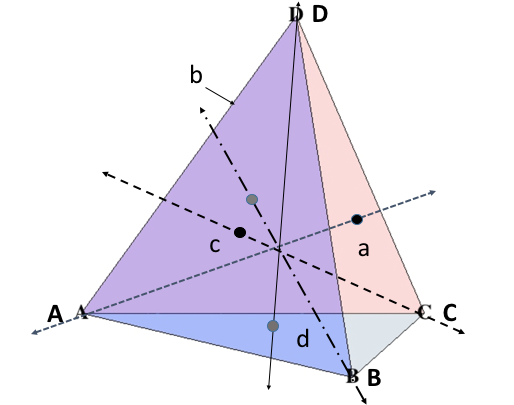
\includegraphics[width=2.5in]{images/TetrahedronC.png}
\caption{\label{fig:TetRot}Tetrahedron with 4 axes of rotation that give symmetries. Figure modified  from \url{https://inspirehep.net/record/1228365/plots}.}
\end{center}
\end{figure}


Each of these axes rotates a triangular face. We'll write one counterclockwise rotation of face $a$ around $\overset{\leftrightarrow}{Aa}$ as $r_{Aa}$ (and similarly for the other axes).
An animation of the rotations of a tetrahedron is available at:

\url{https://www.youtube.com/watch?v=qAR8BFMS3Bc}

You can also make your own tetrahedron like the one in Figure~\ref{fig:TetraFold}.

\begin{figure}[ht]
\begin{center}
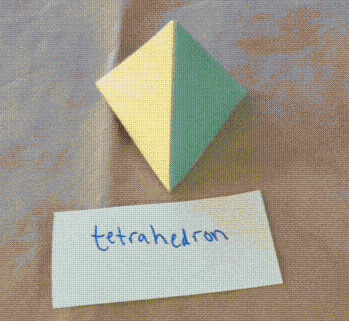
\includegraphics[width=2.5in]{images/TetrahedronFold.png}
\caption{\label{fig:TetraFold}Tetrahedron to print, cut and fold 
(from \url{www.korthalsaltes.com}).}
 
\end{center}
\end{figure}

\begin{exercise}{Tetra 1}
\begin{enumerate}[(a)]
\item How many degrees does $ r_{Aa}$ rotate face $a$?
% 120 degrees
\item What is the order of $r_{Aa}$?
% order 3
\end{enumerate}

\end{exercise}
Consider the tetrahedron in Figure~\ref{fig:TetRot}.  The rotation $r_{Cc}$ takes vertex $D$ to vertex $A$ and face $d$ to face $a$.  

\begin{exercise}{tetra2}
We'll find it useful later to represent these rotations as permutations.
\begin{enumerate}[(a)] 
\item Represent each of the rotations $r_{Aa},$ $r_{Bb},$ $r_{Cc},$ $r_{Dd}$ as permutations on the set of vertices.
\item Represent each of the rotations $r_{Aa},$ $r_{Bb},$ $r_{Cc},$ $r_{Dd}$ as permutations on the set of faces.
\end{enumerate}
\end {exercise}
\begin{exercise}{Tetra3}
\begin{enumerate}[(a)]
\item Give rotations that takes face $c$ to each to each of the other faces $a, b, d$.
\item Give rotations that takes vertex $D$ to each of the other vertices.
\item Consider the edges of the tetrahedron.  Denote the edge between the vertices $C$ and $D$ as $\overline{CD}$: and other edges similarly.  Use this notation to name each of the edges of the tetrahedron.
 \item Give a rotation that takes edge $\overline{CD}$ to each of the other edges.
\end{enumerate}
\end{exercise} 
\begin{exercise}{Tetra4}
Consider the vertex $A$ of a tetrahedron.  What is the equivalence class of this vertex under $G$-equivalence, where $G$ is the groups of rotational symmetries of a tetrahedron?   (Note:  This $G$-equivalence class is the same as orbit of $A$. which we denote as ${\cal O}_A$.)
\end {exercise}

%$ cal{O}_A =\{A,B,C,D\}

Just as with the cube, the rotation group $G$ of any polyhedron acts on the set $X=\{\text{faces}\}\cup\{\text{edges}\}\cup\{\text{vertices}\}$. Recall that each group element $g\in G$ has a \emph{fixed point set} $X_g\in X$ that it leaves unchanged: that is, $gx=x$ for any $x\in X_g$. Let's find some fixed point sets for rotations of the tetrahedron.

\begin{exercise}{Tetra5}
\begin{enumerate}[(a)]
\item Let $G$ be the rotational symmetries of a tetrahedron what is the fixed point set of $r_{Bb}$
%$X_{r_{Bb}}=\{B,b\}
\item What is the fixed point set of $r_{Bb}\compose r_{Dd}$? 
\hyperref[sec:actions:hints]{(*Hint*)}
%$X_{ r_{Bb}\compose r_{Db }}=\{A,a\}$
\item What is the fixed point set of $r_{Bb}^{-1}\compose r_{Dd}$?
\item Give all rotations that fix the set $\{D,d\}$. 
%\item Give a rotation that fixes the following set}{\overline{AB},\overline{CD}\}
\end{enumerate}
\end {exercise}

Let's consider the stabilizer subgroups for the faces and vertices of a tetrahedron. 

\begin{exercise}{Tetra5a}
Find the stabilizer subgroups for each of the following:
$G_{A},  G_{B}$, $G_{C}$, $G_{D}$, $G_{a}$, $G_{b}$, $G_{c}$, $G_{d}$. Which subgroups are equal?
\hyperref[sec:actions:hints]{(*Hint*)}
\end{exercise}

Let's use the stabilizer subgroups above to determine the total number of rotational symmetries of a tetrahedron.  

\begin{exercise}{Tetra6} 
Let $G$ be the rotational symmetries of a tetrahedron.  As in Example~\ref{example:actions:CountingFormula1} construct a formula for $|G|$ in terms of $| G_{A}|$ and $|{\cal O}_{A}|$.  \end {exercise}
So far we've found 4 rotational axes and two rotations around each axis (besides the identity). This gives nine rotations.  As we can see there must be more rotational symmetries of a tetrahedron than we've discovered so far.  Let's try to find them. 

\begin{exercise}{Tetra7}
\begin{enumerate}[(a)]
\item Find the stabilizer subgroup for the edge $\overline{CD}$. 
\item Find the stabilizer subgroup for the edge $\overline{AB}$.
\item How many different group elements (besides the identity) stabilize at least one edge?
\item Are there any group elements that are not stabilizers of either an edge or a face?  Explain your answer.
\end{enumerate}
\end{exercise}	

\begin{exercise}{Tetra8}
In Exercise~\ref{exercise:actions:Tetra6} we constructed a formula for $|G|$ in terms of$| G_{A}|$ and $|{\cal O}_{A}|$.  Can you do the same thing using $| G_{\overline{AB}}|$ and $|{\cal O}_{\overline{AB}}|$?
\end{exercise}

\begin{exercise}{Tetra9}
Complete the following table (similar to the table in Exercise~\ref{exercise:actions:Stabilizers2})to characterize the group elements of the rotational symmetries of a tetrahedron according to the type(s) of sets they stabilize.  We show two rows: fill in the blanks, and add as many rows as necessary to complete the table.
  
\begin{tabular}{| c |c|c| r |} \hline
 \textbf{ Number of group elements} & \textbf{Order} & \textbf{Fixed point set} \\ \hline
  1&  --& entire tetrahedron (identity) \\ \hline
  -- & 3& vertex + face \\   
\end{tabular}

\end{exercise}
% begin{tabular}{ l c r }\begin{tabular}{| c |c|c| r |} \hline
%  \textbf{ Number of group elements} & \textbf{Order} & \textbf{Fixed point set} \\ \hline
  %Number of elements & order of the element & Type of set that it stabilizes \\
% 1 & 1 & entire tetrahedron (identity) \\
  %8 & 3 & vertex+face \\
 % 3 & 2 & edge \\
%\end{tabular}
\begin{exercise}{}
Recalling Exercise~\ref{exercise:actions:Stabilizers2b}, we may suppose that there is a permutation group which resembles the symmetry group of the tetrahedron, in the same way that $S_4$ resembles the symmetry group of the cube. Identify a well-known symmetry group with 12 elements and  make a table for this group which is arranged like the table in Exercise~\ref{exercise:actions:Stabilizers2b}. What do you conjecture based on your results?
\end{exercise}
\subsubsection*{The octahedron}
Another regular polyhedron is the octahedron.  We will see that in some ways an octahedron is like a cube. 
When opposite points are lined up  on a vertical $z$ axis, the octahedron has no vertical or horizontal faces, as shown in Figure~\ref{fig:OctaRot}.  We denote a  $90^{\circ}$ counterclockwise rotation around the $z$ axis by $r_z$ (and similarly for rotations around the $x$, and $y$ axes).
Since each vertex of the octahedron lies on an axis, we can use the $x,y$, and $z$ axis to label the vertices.  For example $y_+$ is the vertex on the positive $y$ axis.   We can also name the edges using this notation for their endpoints.   Let's use the axes to label the faces of the octahedron too.  Consider Figure~\ref{fig:OctaRot}, we'll refer to the the face in the first octant as $\triangle_{ +++}$ (the other faces will be labeled similarly).

\begin{figure}[ht]
\begin{center}
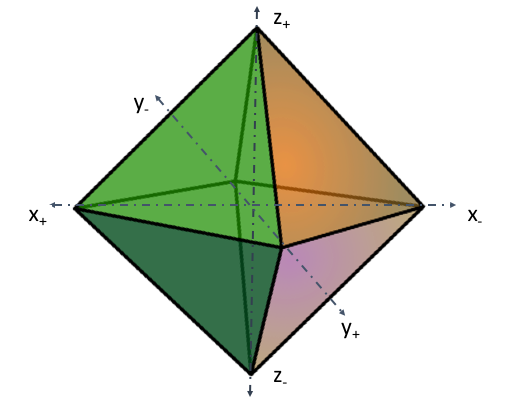
\includegraphics[width=2.5in]{images/AxesOfOctahedron.png}
\caption{\label{fig:OctaRot}Octahedron with 3 axes of rotation that give symmetries (figure modified from \url{https://en.wikipedia.org/wiki/File:Octahedron.svg})
}
\end{center}
\end{figure}


\begin{exercise}{Octa1}
\begin{enumerate}[(a)]
\item List all the faces of the octahedron using the notation above.
\item Based on Figure~\ref{fig:OctaRot}  how many faces does an octahedron have? How many vertices?  How many edges?
\end{enumerate}
%8 faces, 12 edges, 6 vertices
\end {exercise}

A model of an octahedron might help with the following exercises.  You can make one like the one in Figure~\ref{fig:OctaFold}. There's also a virtual octahedron on GeoGebra that you can manipulate at: 
\url{https://www.geogebra.org/m/KtTGGrSp}.  A Youtube video that shows the rotational symmetries of an octahedron may be found at:
\url{https://www.youtube.com/watch?v=CCaX5eTteEg}.

\begin{figure}[ht]
\begin{center}
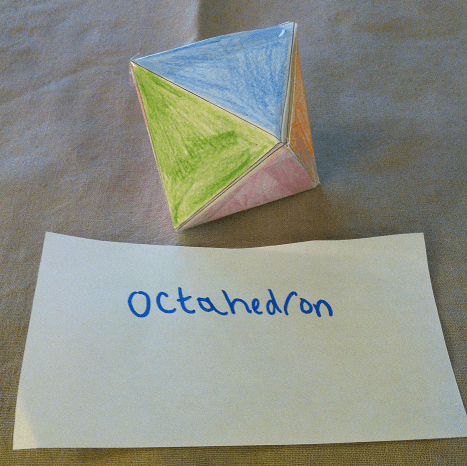
\includegraphics[width=2.5in]{images/OctahedronFold.png}
\caption{\label{fig:OctaFold} A paper octahedron to print, cut and fold
 (from \url{www.korthalsaltes.com}). }

\end{center}
\end{figure}

\begin{exercise}{Octa2}
What is the order of $r_z$?
%$|r_z|=3$
\end{exercise}

\begin{exercise}{Octa3}
\begin{enumerate}[(a)]
\item Give rotations that take $\triangle _{+++}$ to each to each of the other faces.
\item Give rotations that take  $x_-$ to each of the other vertices.
\item Give a rotation that takes edge $\overline{z_+y_+}$ to each of the other edges.
\end{enumerate}
\end{exercise} 
\begin{exercise}{Octa4}
Consider the edge $\overline{x_-y_+}$ of a octahedron. What is ${\cal O}_{\overline{x_-y_+}}$?
\end {exercise}

\begin{exercise}{Octa5}
Let $G$ be the rotational symmetries of an octahedron
\begin{enumerate}[(a)]
\item  What is the fixed point set of $r_{y}\compose r_{z}$?
%$X_{r_{y}\compose r_{z}}=\{x_+,x_-\}$
\item What is the fixed point set of $r_{y}^2\compose r_{x}$? 
%$X_r_{y}^2\compose r_{x}=\{\overline {y_+z_+},\overline{y_-z_-}\}$
\item What is the fixed point set of $r_{x}^2\compose r_{y}$?
\end{enumerate}
\end {exercise}

Let's consider the stabilizer subgroups for the faces and vertices of an octahedron.  
 
\begin{exercise}{Octa5a}
Find the stabilizer subgroups for each of the vertices of the octahedron. 
\hyperref[sec:actions:hints]{(*Hint*)}
\end{exercise}

Let's find the total number of rotational symmetries for the octahedron. 

\begin{exercise}{Octa6} 
Let $G$ be the rotational symmetries of an octahedron. Construct a formula for $|G|$ in terms of $| G_{y_+}|$ and $|{\cal O}_{y_+}|$ (see Example~\ref{example:actions:CountingFormula1}).
 \end {exercise}

So far we have discovered 10 rotational symmetries of an octahedron.  Three axis of 3 rotations each plus the identity.  By the previous exercise, there are still more to discover.  Here we go! 

\begin{exercise}{Octa7}
\begin{enumerate}[(a)]
\item Find the stabilizer subgroup for the edge $\overline{y_+~z_+}$. 
\item Find the stabilizer subgroup for the edge $\overline{y_-~z_-}$.
\item How many different group elements (besides the identity) stabilize at least one edge?
\end{enumerate}
\end{exercise}	

\begin{exercise}{Octa8}
\begin{enumerate}[(a)]
\item Find the stabilizer subgroup for the face $\triangle_{+ + +}$.
\item Find the stabilizer subgroup for the face $\triangle_{ -~-~-}$.
\item How many different group elements stabilize at least one face?
\end {enumerate}
\end{exercise}

\begin{exercise}{Octa9}
In Exercise ~\ref {exercise:actions:Octa6} we constructed a formula for $|G|$ in terms of $|G_{y_+}|$ and $|{\cal O}_{y_+}|$.  Can you do the same thing using $|G_{\triangle_{+ + +}}|$ and $|{\cal O}_{\triangle_{+ + +}}|$?
\end{exercise}

\begin{exercise}{Octa10}
Complete the following table to characterize the group elements of the rotational symmetries of an octahedron.  We show two rows, how many more to complete the table? 
 
\begin{tabular}{| c |c|c| r |} \hline
 \textbf{ Number of group elements} & \textbf{Order} & \textbf{Fixed point set} \\ \hline
  ---&  ---& entire  octahedron (identity) \\ \hline
  --- & ---&  opposite vertices \\

\end{tabular}
\end{exercise}
% begin{tabular}{ l c r }
  % \textbf{ Number of group elements} & \textbf{Order} & \textbf{Fixed point set} \\ \hline
% 1 & 1 & entire octahedron (identity) \\
%6 & 4  & opposite vertices\\
% 3 & 2 & opposite vertices\\
  %8 & 3 & opposite faces  \\
 % 6 & 2 & opposite edges \\
%\end{tabular}

\begin{exercise}{dual}
There are some striking similarities between the tables in Exercises~\ref{exercise:actions:Octa10} and \ref{exercise:actions:Stabilizers2}. Describe the similarities, and see if you can explain them. Figure~\ref{fig:Dual} may give you some ideas.
\end{exercise}

\begin{figure}[ht]
\begin{center}
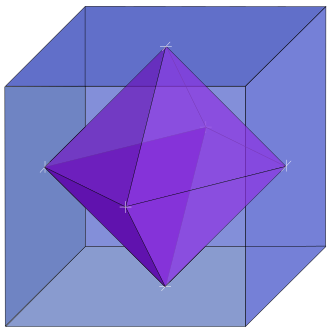
\includegraphics[width=2.5in]{images/Dual_Cube-Octahedron.png}
\caption{\label{fig:Dual}Figure for Exercise~\ref{exercise:actions:dual} (source: \url{https://en.wikipedia.org})}

\end{center}
\end{figure}

\subsubsection*{The dodecahedron}
Let's practice finding the elements of the rotation group of another regular polyhedron.  Consider the regular dodecahedron in Figure~\ref{fig:Dodeca}.  A dodecahedron has 12 faces and each face is a regular pentagon.  How many edges does this polyhedron have and how many vertices?  Well, since each of the twelve faces is a pentagon that seems to give $12\cdot 5=60$ edges.  But two faces meet at each edge, so we actually have $(12\cdot 5)/2=30$ edges.

\begin{figure}[ht]
\begin{center}
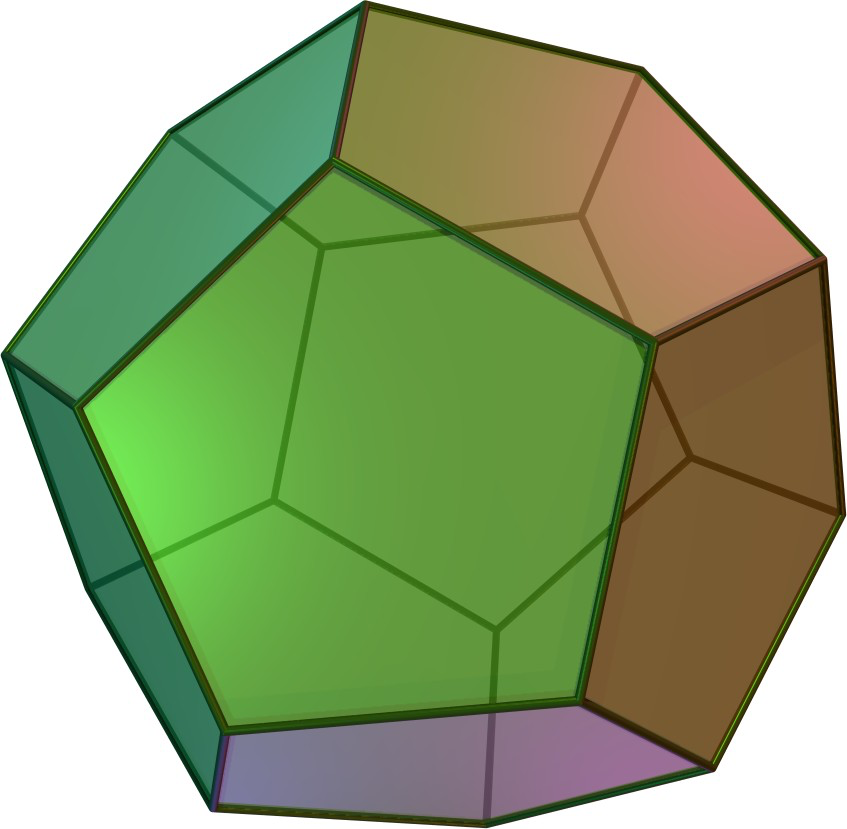
\includegraphics[width=2.5in]{images/Dodecahedron.png}
\caption{\label{fig:Dodeca}Dodecahedron (source:\url{https://en.wikipedia.org})}

\end{center}
\end{figure}

You can also make your own dodecahedron to help you explore its rotational symmetries. See Figure~\ref{fig:DodecaFold}.

\begin{figure}[ht]
\begin{center}
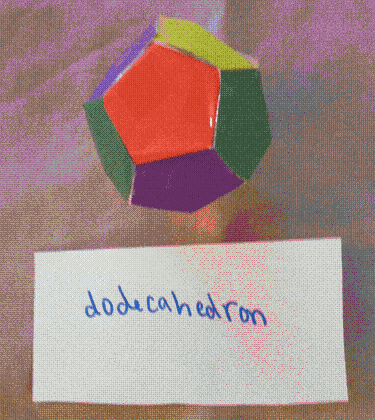
\includegraphics[width=2.5in]{images/DodecahedronFold.png}
\caption{ \label{fig:DodecaFold}A dodecahedron to print, cut and fold  (from  \url{www.korthalsaltes.com}).}

\end{center}
\end{figure}

\begin{exercise}{Dodeca1}
Determine the number of vertices of a regular dodecahedron.
\end{exercise}
Let $f_1$ be one face of the dodecahedron.  An axis through the center of $f_1$ also passes the opposite face which is parallel to $f_1$. We'll call this opposite face $f_1^*$ and denote a counterclockwise rotation of $f_1$ about this axis as $r_{f_1}$.

\begin{exercise}{Dodeca2}
\begin{enumerate}[(a)]
\item What is the order of $r_{f_1}$?
% order 5
\item Let $G$ be the rotational symmetry group of a dodecahedron.  List all rotations in the stabilizer subgroup $G_{f_1}$.  What else do they stabilize?
%$G_{f_1}={\var{id},r_{f_1},r_{f_1}^2, r_{f_1}^3, r_{f_1}^4}$, $G_{f_1}$ will also stabilize the opposite (parallel) face.
\item What is $|G_{f_1}|?$
% $|G_{f_1}|=5$
\item How many group elements in $G$ stabilize at least 1 face?
%25 elements 4 rotations for each of 6 pairs of opposite faces, plus the identity.
\item What is $|{\cal O}_{f_1}|$?
%$|{\cal O}_{f_1}|=12$ The orbit of $f_1$ includes all faces of the dodecahedron.
\end{enumerate}
\end{exercise}
Now we can find the total number of rotational symmetries in $G$.

\begin{exercise}{Dodeca3}
Find $|G|$ in terms of $|G_{f_1}|$ and $|{\cal O}_{f_1}|$.
%$5\times 12=60$
\end {exercise}
So far we've found the number of the stabilizers of faces of the dodecahedron.  But, as with the cube and tetrahedron, we need axes of symmetry through edges and vertices as well.
Let $v_1$ be one vertex of the dodecahedron.  An axis of symmetry through $v_1$ will also pass through the opposite vertex, which we will call $v_1^*$.  A counterclockwise rotation about this axis is called $r_{v_1}$.

\begin{exercise}{Dodeca4}
\begin{enumerate} 
\item Find the order of $r_{v_1}$.
% order 3
\item List all rotations in the stabilizer subgroup $G_{v_1}$.  What else do they stabilize?
%$G_{v_1}={\var{id},r_{v_1},r_{v_1}^2}$ $G_{v_1}$ will also stabilize the opposite vertex.
\item How many group elements in $G$ (besides the identity) stabilize at least 1 vertex?
% 20 rotations 10 pairs of vertices, 2 rotations besides the identity stabilize each pair.
\item What is $|{\cal O}_{v_1}|$?
%$|{\cal O}_{v_1}|=20$ The orbit of $v_1$ includes all the vertices of the dodecahedron.
\item Find $|G|$ in terms of $|G_{v_1}|$ and $|{\cal O}_{v_1}|$.
\end{enumerate}
\end{exercise}
Let's consider the edges of the dodecahedron.  We've seen already that there are 30 edges.  Based on this information and previous exercises, complete the following.

\begin{exercise}{Dodeca5}
\begin{enumerate}[(a)]
\item Let $e_1$ be one edge of the dodecahedron. What is $|G_{e_1}|$?
%2
\item Are the edges of a dodecahedron stabilized in pairs?  Explain your answer.
\hyperref[sec:actions:hints]{(*Hint*)}
% There are 60 group elements in $G$.  By previous exercise 25 elements stabilize faces, 20 rotations stabilize vertices. We need 15 more elements to make up $G$.  There are $30/2=15$ pairs of edges, so edges must come in pairs.
\end{enumerate}
\end{exercise}

\begin{exercise}{Dodeca6} 
\begin{enumerate}[(a)]
\item How many group elements of $G$ besides the identity stabilize at least 1 edge?
% 15, one rotation for each pair of edges.
\item
Complete the following table to characterize the group elements of the rotational symmetries of a dodecahedron.  We show two rows, how many more to complete the table?  

\begin{tabular}{| c |c|c| r |} \hline
 \textbf{ Number of group elements} & \textbf{order} & \textbf{Fixed point set} \\ \hline
  --&  --& entire  dodecahedron (identity) \\ \hline
  -- & --&  -- \\ 
\end{tabular}
\end{enumerate}
\end{exercise}
% begin{tabular}{ l c r }
%\textbf{ Number of group elements} & \textbf{order} & \textbf{Fixed point set} \\ \hline
% 1 & 1 & entire dodecahedron (identity) \\
%24 & 5 & opposite faces  \\
% 15 & 2 & opposite edges \\
%20 & 3  & opposite vertices\\
\begin{exercise}{}

Identify a group of permutations with the same number of elements as the symmetry group of the dodecahedron. Make a table for this group which is arranged like the table in Exercise~\ref{exercise:actions:Stabilizers2b}. What do you conjecture based on your results?
\end{exercise}

\subsubsection*{Football (a.k.a. ``soccer ball'')}
All the polyhedra we've studied so far have congruent regular faces.  These are also known as \term{Platonic solids}\index{Platonic solids}.  Let's explore the rotation group of a polyhedron whose faces are not all congruent.  A familiar example is the football (following 
American usage, we'll call it a``soccer ball'), as shown in  Figure~\ref{fig:Soccer}\index{Soccer ball}.  The soccer ball has 32 faces, 12 regular pentagons and 20 hexagons.  

\begin{figure}[ht]
\begin{center}
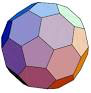
\includegraphics[width=2in]{images/Soccerball.png}
\caption{The soccer ball has both pentagonal and  hexagonal faces.  Source: \url{http://mathworld.wolfram.com/TruncatedIcosahedron.html}.
}
\label{fig:Soccer}
\end{center}
\end{figure}

Let's try to count the rotations of a soccer ball that preserve symmetry.  Axes can be placed through the center of pentagonal faces, which are stabilized in pairs. 

\begin{exercise}{Soccer1}
\begin{enumerate}[(a)]
\item
Given one particular pentagonal face of the soccer ball, what is the order of its stabilizer?
\item
Given that there are 12 pentagonal faces, find $|G|$ where $G$ is  group of rotational symmetries of the soccer ball.
\hyperref[sec:actions:hints]{(*Hint*)}
\end{enumerate}
\end {exercise}

 Axes can also be placed through the center of hexagonal faces.  However, not all rotations about an axis through a hexagonal face will result in symmetry.

\begin{exercise}{Soccer2}
\begin{enumerate}[(a)]
\item
Given one particular hexagonal face of the soccer ball, what is the order of its stabilizer?
\item
Using your answers to (a) and part (b) of Exercise~\ref{exercise:actions:Soccer1}, determine the number of hexagonal faces. \hyperref[sec:actions:hints]{(*Hint*)}
\end{enumerate}
\end {exercise}

Axes of rotation also pass through \emph{some} of the edges. Notice that there are two types of edges: those which join two hexagonal faces, and those which join a hexagonal face and a pentagonal face.

\begin{exercise}{Soccer3}
\begin{enumerate}[(a)]
\item
Consider an edge which joins a hexagonal face and a pentagonal face. How many rotations (besides the identity) stabilize this edge?  \emph{Explain} your answer.
\item
Consider an edge which joins two hexagonal faces. How many rotations stabilize this edge?  \emph{Explain} your answer.
\item
Using the counting formula and your answers to previous exercises, determine the number of edges which join  two hexagons.
\item
Note each pentagon touches 5 hexagons. Use this information and information from Exercise~\ref{exercise:actions:Soccer1} to determine the number of edges which join a pentagon and hexagon.
\end{enumerate}
\end {exercise}

What about vertices?

\begin{exercise}{Soccer4}
\begin{enumerate}[(a)]
\item
Consider a particular vertex. How many rotations (besides the identity) stabilize this edge?  \emph{Explain} your answer.
\item
Note each vertex touches one pentagon, and each pentagon has five vertices. Use this information and information from Exercise~\ref{exercise:actions:Soccer1} to determine the number of vertices.
\end{enumerate}
\end {exercise}

\begin{exercise}{Soccer5}
\begin{enumerate}[(a)]
\item
Create a table similar to the table in Exercise~\ref{exercise:actions:Stabilizers2} which characterizes the rotational symmetries of the soccer ball.
\item
Does this table resemble one of the tables that we constructed previously for regular polyhedra? If so, which? Can you explain this?
\end{enumerate}
\end {exercise}


\subsection{Euler's formula for regular polyhedra}\label{sec:actions:Euler}
In this section we'll play with counting the order of the rotation group $G$ of a regular polyhedron in different ways. It turns out that this will lead us to an interesting and useful formula relating the number of edges, vertices, and faces in a polyhedron.
Let's start by reviewing our previous examples and noticing a pattern.

\begin{exercise}{Eulers1}
\begin{enumerate}[(a)]
\item
Complete the table and compare $|G|$ to the number of edges of each polyhedron.  The number of edges is equal to the order of the orbit of any edge $e$, denoted as $|{\cal O}_e|$.

\begin{tabular}{|c | c | c|}\hline
polyhedron & number of edges ($|{\cal O}_e|$) & order of group ($|G|$)\\ \hline
cube &  12 &   24\\ \hline
tetrahedron &  -- &   --\\ \hline
octahedron & -- &--\\ \hline
dodecahedron &  --&--\\ \hline 
\end{tabular}
\item Based on the table, guess an equation for $|G|$ in terms of ${\cal O}_e$.
\item 
Prove your equation using Proposition~\ref{proposition:actions:CountingFormula}.
% $|G|=2\cdot |{\cal O}_e|\$
\end{enumerate}
\end {exercise}
 Now in Exercises~\ref{exercise:actions:Stabilizers2}, \ref{exercise:actions:Tetra9}, and \ref{exercise:actions:Octa10}  we showed another way of counting the elements of $G$: by counting the stabilizers of faces, vertices, and edges (plus the identity)But does this work for \emph{every} polyhedron? Could there possibly be a rotation that doesn't stabilize \emph{anything}? It turns out that this isn't possible (at least in three dimensions). The argument (which depends on a key fact proved by the famous mathematician Leonhard Euler) goes as follows. 

Euler proved in 1775 that any rotation in three dimensions has a unique fixed axis. (We won't give the proof here, but it's related to the cross product discussed in Section~\ref{subsec:LeviCivita}.)  Now if we  rotate a polyhedron, then the axis must intersect the polyhedron twice: that is, it must intersect two elements of $X$ where $X = \{\text{faces, vertices, edges}\}$. Let's call these two elements $\epsilon_1$ and $\epsilon_2$. Since the rotation leaves the two intersections unchanged, there's one point of $\epsilon_1$ which maps to itself (and similarly for $\epsilon_2$). If the rotation is a symmetry, then $\epsilon_1$ must be fixed by the rotation, because there's no way it couldn't map to a different element of $X$ and still have one point which remains in $\epsilon_1$. The same argument holds for $\epsilon_2$. This shows that any rotational symmetry must stabilize at least two elements of $X$. 

We can take the argument even further. The rotational symmetry which stabilizes $\epsilon_1$ and $\epsilon_2$ can't possibly stabilize any other elements of $X$: this is because the center point of any stabilized element (be it face, vertex, or edge) is unchanged by a rotational symmetry, and Euler tells us that there is only one fixed axis and hence exactly two fixed points.  

So since every rotational symmetry (besides the identity) stabilizes \emph{exactly} two elements, then if we sum up all of the (non-identity) stabilizers for all elements of $X$ then we will count each (non-identity) symmetry exactly twice. It follows that
\[ 2(|G|-1) = \sum_{x \in X}  (|G_x|-1) \]
(note that we use $|G|-1$ and $|G_x|-1$  because we're not counting the identity symmetry). 


Let's apply this formula to a regular polyhedron with $|{\cal O}_f|$ faces, $|{\cal O}_v|$ vertices and $|{\cal O}_e|$ edges.  Applying Proposition~\ref{proposition:actions:CountingFormula} to faces, edges, and vertices gives:
\[ |G_f|=\frac{|G|}{|{\cal O}_f|}; \qquad |G_e|=\frac{|G|}{|{\cal O}_e|}; \qquad |G_v|=\frac{|G|}{|{\cal O}_v|}.\]
Now for the sum.  Since there are ${\cal O}_f$ faces, ${\cal O}_e$ edges, and ${\cal O}_v$ vertices we have:
\begin{align*}
2 (|G| -1) &=  \sum_{x \in X}  (|G_x|-1)\\
&=  \sum_{\text{faces}}  (|G_f|-1)+\sum_{\text{edges}}  (|G_e|-1)+\sum_{\text{vertices}}  (|G_v|-1)\\
&= |{\cal O}_f|  \left(\frac{|G|}{|{\cal O}_f|}-1\right)+ |{\cal O}_e| \left(\frac{|G|}{|{\cal O}_e|}-1\right)+  |{\cal O}_v|\left(\frac{|G|}{|{\cal O}_v|}-1\right)\\
&=  3|G| - |{\cal O}_f| -  |{\cal O}_e| -  |{\cal O}_v|.
\end{align*}
Rearranging, we find:
\[ |{\cal O}_f| +  |{\cal O}_v|  +  |{\cal O}_e| =  |G|+2. \]
But we've also seen that $|G| = 2{\cal O}_e$ for regular polyhedra. Substituting and rearranging a little further gives:
\[ |{\cal O}_f|+|{\cal O}_v|-|{\cal O}_e|=2. \]
This powerful equation is a special case of \term*{Euler's formula}\index{Euler's formula!For networks on a sphere}.  Let's see how it can be useful in determining properties of regular polyhedra.

\begin{exercise}{Euler5}
A certain regular polyhedron has 20 triangular faces. 
\begin{enumerate}[(a)]
\item
Using Proposition~\ref{proposition:actions:CountingFormula}, find the number of edges.
\item
Using Euler's formula, find the number of vertices.
\item
Using Proposition~\ref{proposition:actions:CountingFormula}, find the number of edges which meet at each vertex.
\end{enumerate}
\end {exercise}

\begin{exercise}{Euler 4}
\begin{enumerate}[(a)]
\item Verify Euler's formula for the cube and tetrahedron.
\item Explain why the proof we have given does not apply to the soccer ball. Verify that notwithstanding, Euler's formula still works for the soccer ball anyway! 
\end{enumerate}
\end {exercise}


It turns out that this version of Euler's formula works for any network of edges and vertices which can be drawn on a sphere. Variants of the formula work for networks drawn on other shapes (like a donut).  Pursuing this topic further would lead us into the area  of mathematics known as \term{algebraic topology}, which is utterly fascinating but unfortunately a bigger mouthful than we can chew at this point. 

We don't need to limit ourselves to Euler's formula.  There are lots of other fun facts we can prove:

\begin{exercise}{Euler n}
\begin{enumerate}[(a)]
\item Modify the proof of Euler's formula to prove the following formula for the soccer ball:
\[2 =  |\text{faces}| + |\text{edges}| + |\text{vertices}| - X \cdot |G|,\]
where $|G|$ is the order of the symmetry group of the soccer ball.  Find the value of $X$.
\item 
Prove that the following formula is true for \emph{any} network of edges and vertices which can be drawn on a sphere:
\[ |\text{faces}| + |\text{edges}| + |\text{vertices}| -2 \equiv 0 \pmod{|G|},\]
where $|G|$ is the order of the rotational symmetry group of the network.
\end{enumerate}
\end{exercise}


\begin{exercise}{FunFact}
Let $X$ be a polyhedron consisting of faces, edges and vertices. The symmetry group of $X$ is $G$. $X$ is not a regular polyhedron--the vertices and edges are not all identical.  This is what we know about $X$:
\begin{itemize}
\item
There are two types of vertices, and two types of edges. 
\item Type I vertices are all $G$-equivalent; and every Type I vertex has 5 edges which are all $G$-equivalent. (This implies that the stabilizer subgroup of any Type I vertex has order 5.)
\item Type II vertices are all $G$-equivalent.
\item Type I edges are all $G$-equivalent; and the 180-degree rotation about the axis through the origin and the center of any Type I edge is a symmetry. (In other words, the stabilizer subgroup  of any Type I edge has order 2.)
\item Type II edges are all $G$-equivalent; and Type II edges are not fixed by any symmetries.
\item All faces are triangles, and all are $G$-equivalent.
\end{itemize}
\begin{enumerate}[(a)]
\item 
Use the Counting Formula (Proposition~\ref{proposition:actions:CountingFormula}) to express the number of Type I vertices, Type I  edges, and Type II edges in terms of $|G|$.
\item 
Prove that $|G|$ is divisible by 10.
\item
Since every edge is shared by two faces, it follows that:
\[ 2 \cdot \text{(number of edges) = (number of faces)(number of edges per face)}.\]
Use this fact to express the number of faces in terms of $|G|$.
\item
Compute the order of the stabilizer subgroup of any face in $X$.
\item
Use Euler's formula to express the number of Type II vertices in terms of $|G|$.
\item
Using the Counting Formula applied to Type II vertices, show that the order of the stabilizer subgroup of any Type II vertex is 3 or less. Then show that  order 1 and order 2 are both impossible, so that the order must be 3.
\item
Using Euler's formula, compute $|G|$. Give explicitly the number of vertices and edges of each type, and the number of faces.
\item
Look up on the web, and see if you can identify this polyhedron (this is an example of an \term{Archimedian solid}).
\end{enumerate}
\end{exercise}

\subsection{Are there  other regular polyhedra?}

We have investigated four regular polyhedra: cube, tetrahedron, octahedron, and dodecahedron.  Could there be any others?  What does group theory tell us? 


\begin{exercise}{allPoly}
Let us suppose we have a regular polyhedron with $n_f$ faces, $n_e$ edges, and $n_v$ vertices.  Let us further suppose that each face has $f$ edges per face and $v$ edges which meet at each vertex. (Note in particular that $v \ge 3$, because 2 parallel edges which join together form a single edge and not a vertex.) Let $G$ be the group of rotational symmetries.
\begin{enumerate}[(a)]
\item
Use the Counting Formula to obtain three different equations for $|G|$ in terms of $n_f, n_e, n_v, f$, and $v$.
\item
Use part (a) and Euler's formula to find an equation that relates $f, v$, and $|G|$ (that is, these are the only 3 variables in the equation).
\item
Suppose that $f=3$.  Find the possible values of $v$.  For each value of $v$, find the corresponding values of $|G|, n_f, n_e$, and $n_v$.
\item
Suppose that $f=4$.  Find the possible values of $v$.  For each value of $v$, find the corresponding values of $|G|, n_f, n_e,$ and $n_v$.
\item
Suppose that $f=5$.  Find the possible values of $v$.  For each value of $v$, find the corresponding values of $|G|, n_f, n_e,$ and $n_v$.
\item
Suppose that $f \ge 6$. Show that this would imply $v<3$, which is impossible.
\item
Besides the four polyhedra we have investigated, could there be any others? If so, what are its properties?
\end{enumerate}
\end{exercise}

Take a moment to appreciate how amazing these results are.  Since polyhedra are geometrical objects, one would think that one would have to consider geometrical facts about angles and how they fit together in order to determine which ones are possible.  In particular, we know from geometry that a regular polyhedron couldn't have more than 6 regular polygons meeting at an edge, because then we'd have more than 360 degrees. Geometry also tells us that polyhedral faces couldn't have more than 6 sides, since then we couldn't have more than 2 meeting at a vertex. But we have figured out which regular polyhedra can exist, purely on the basis of algebra with no considerations of angles whatsoever!  

The other wonderfully mysterious fact is that all of the regular polyhedra that we have determined to be possible do actually exist. It seems that our simple algebraic representations  have captured some deep properties of the three-dimensional world that we live in.

\subsection{Reflection symmetries of polyhedra}\label{subsec:reflSym}
We have never shown that the rotational symmetries are the \emph{only}  symmetries of the regular solids In fact, there are others! Recall that in the dihedral group, besides rotations there were reflections. Consider for example the hexagon: it had 6 rotations (including the identity) and 6 reflections. It's possible to rotate the hexagon and keep the hexagon in the same plane. However, to reflect the hexagon, you have to ``flip'' it, which requires three dimensions.  It turns out that something similar is true for the regular solids. There are also reflection symmetries for the regular solids: in fact, there are as many reflections as rotations, just as in the dihedral group. Also like the dihedral group, to reflect a solid requires one extra dimension. It is rather mind-blowing to think that if we lived in a world with four physical dimensions, it would be possible to turn your right hand into your left hand just by ``flipping'' in the fourth dimension!

\subsection{Finite subgroups of the group of rotations in 3 dimensions}
The set of all possible rotations in 3 dimensions forms a group, which is called the \term{special orthogonal group} and is denoted by the symbol $SO_3$. ($SO_3$ is actually the intersection of the ``orthogonal group'' $O_3$ with the special linear group in three dimensions, which is why it's called ``special''.)  All of  the rotational symmetry groups of regular polyhedra which we've been considering are finite subgroups of  $SO_3$. 

In Chapter~\ref{symmetries} we encountered another class of finite subgroups of $SO_3$, namely the dihedral groups $D_n$ which consist of rotations and flips (we should be careful to include $D_2$, which is generated by  a single 180-degree rotation and a flip). Although a flip is not a 2-d rotation, it is a rotation in 3-dimensions (as we indicated in  Section~\ref{subsec:reflSym}). Naturally, the rotation groups for the different $n$-gons (which are subgroups of the $D_n$ form another class of finite subgroups of $SO_3$.

Are there any other finite subgroups of $SO_3$.  The answer is \emph{NO}-- and we can prove it! For a proof, the reader may consult: \url{hompages.math.uic.edu/~kauffman/FiniteRot.pdf}.

Once again, note the amazing power of mathematics. Mathematics commands the universe, and it must obey. Mathematics tells reality what it can and cannot do.


\section{Conjugation}\label{Conjugation}
\subsection{Commutative diagrams and the definition of conjugation}
When we talked about permutations, we saw that the objects we were permuting didn't really change the situation.  For example, we saw that permuting $\{1,2,3,4\}$ was the ``same thing'' as permuting $\{A,B,C,D\}$. Now what do we really mean by the ``same thing''? Well for example, if we take any permutation of $\{1,2,3,4\}$ and replace $1$ with $A$, $2$ with $B$ and so on, then we'll get a permutation of $\{A,B,C,D\}$. To be specific let's take $\sigma=(123)$ and $f=\begin{pmatrix} 1&2&3&4\\A&B&C&D\end {pmatrix}$.  It's possible to represent this situation with diagram in Figure~\ref{fig:Commutative1}. This type of diagram is called a \term{commutative diagram}.\index{Commutative!diagram}


The commutative diagram illustrates the construction of a conjugation. We can begin in the upper right corner and move to the upper left, in the opposite direction of the $f$ arrow. This motion corresponds to
applying the inverse of $f$, that is 
 $f^{-1}$ (this naturally requires that $f$ must be a \emph{bijection}).  Then, moving from upper left to lower left represents applying the permutation $\sigma=(123)$, as shown in the diagram.  Finally, by moving from lower left to lower right (which corresponds to 
applying the function $f$), we end up at the lower right-hand corner. The three motions, performed one after the other thus corresponds to the composition of functions $f^{-1}$, then $\sigma$, then $f$, which we write as
$f \sigma f^{-1}$ (recall that function composition proceeds from right to left). 

On the other hand, moving directly from upper right to lower right corresponds to the application of 
the permutation $\mu$. Since this motion starts at upper right and ends at lower right just like the previous
one, it should represent the same permutation as before. This gives us the result:
 $\mu=f\sigma f^{-1}$.    

\begin{figure}[ht]
\begin{center}
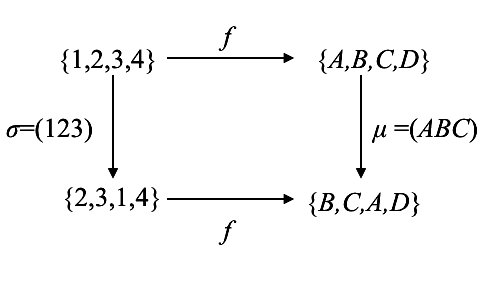
\includegraphics[width=2.5in]{images/Commutative1.png}
\caption{Commutative diagram of a conjugate mapping.}\label{fig:Commutative1}
\end{center}
\end{figure}

We may also think of this another way. The paths $f\sigma$ and $\mu f$  both take us from upper left to lower right. 
 So we can write $f\sigma$= $\mu f$. By right multiplying by $f^{-1}$ we discover the algebraic structure of the conjugate of $\sigma$,  $f\sigma f^{-1}=\mu$. 
 
There's a shortcut way to obtain $\mu$. Actually, $\mu$ is simply $\sigma$ relabeled according to $f$.  That is, if we take the cycle representation of $\sigma$ and replace the numbers according to $f$ ($1\rightarrow A, 2\rightarrow B, 3\rightarrow C$), then we end up with $\mu$.  We will call this shortcut, ``the relabeling method''.\index{Conjugation!relabeling method}

\begin{exercise}{Conj1}
For each $\sigma$ and and $f$, complete a commutative diagram like the one in Figure~\ref{fig:Commutative1}. Find the conjugate mapping in two ways, using conjugation and the relabeling method.
\begin{enumerate}[(a)]
\item $\sigma=(12)(35)$ and $f=\begin{pmatrix} 1&2&3&4&5\\ A&B&C&D&E& \end{pmatrix} $
\item $\sigma=(2346)$ and $f=\begin{pmatrix} 1&2&3&4&5&6\\ A&B&C&D&E&F \end{pmatrix}$
\item $\sigma=(147)(2563)$ and $f=\begin{pmatrix} 1&2&3&4&5&6&7\\ A&B&C&D&E&F&G \end{pmatrix}$
\end{enumerate}
\end {exercise}
Now instead of $f$ going between different sets, we can choose $f$ to map $\{1,2,3,4\}$ to itself. In this case, $f$ itself is a permutation.  To be more consistent with our earlier notation for permutations, we'll use the symbol $\tau$ instead of $f$ in the following discussion.  What $\tau$ corresponds to is just relabeling the objects that we're permuting. Figure~\ref{fig:Commutative2} shows an example where both $\tau$ and $\sigma$ are permutations on the set $\{1,2,3,4\}$. The diagram shows that if we do a permutation $\sigma$ on the originally-labeled objects, and compare to the same permutation of the relabeled objects, we find that the relabeled permutation is exactly given by $\tau\sigma \tau^{-1}$. The permutations $\sigma$ and $\tau\sigma \tau^{-1}$ are called \term{conjugate permutations}\index{Permutation!conjugate}, and the operation which takes $\sigma$ to $\tau \sigma \tau^{-1}$ is called \term{conjugation}.\index{Conjugation!of permutations}\footnote{Note this is quite different from conjugation of complex numbers. Unfortunately, ``conjugation'' is a very popular word in mathematics, and is used in many different senses.}

\begin{figure}[ht]
\begin{center}
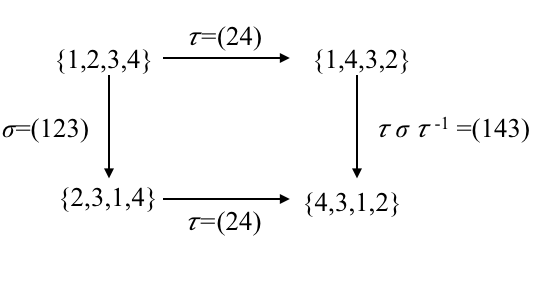
\includegraphics[width=3in]{images/Commutative2.png}
\caption{Conjugate mapping with $\tau$ and $\sigma$ permuting $\{1,2,3,4\}$.}\label{fig:Commutative2}
\end{center}
\end{figure}

\subsection *{Conjugate permutations and cycle structure}

Two permutations that are conjugate are in many ways very similar. We could almost call them the ``same'' permutation, only they act on a relabeled set of objects. In particular, it's true that two conjugate permutations must have the same cycle structure. For instance, in the example we did earlier in Figure~\ref{fig:Commutative1} we saw that both permutations were three-cycles.  This will be true in general because conjugation simply means relabeling the objects that are permuted, without changing anything else.

\begin{example}{Conj2}
Let $\sigma = (153)(276)$ and $\tau = (427)(165)$. Then
$$\tau=\begin{pmatrix} 1&2&3&4&5&6&7\\6&7&3&2&1&5&4  \end{pmatrix}.$$ 
Relabeling $\sigma$ according to $\tau$ gives the conjugate $(136)(457)$. You can check that computing $ \tau \sigma \tau^{-1}$ will give the same result as the relabeling method.
\end{example}
\begin{exercise}{Conj3}
Given $\sigma$ and $\tau$ use the relabeling method to find the permutation conjugate to $\sigma$.  Check your work by computing $\tau\sigma\tau^{-1}$.
\begin{enumerate}[(a)]
\item 
$\sigma=(6247)$ and $\tau=(527)(63)$.  $\sigma$ and $\tau$ act on the set $\{1,2,3,4,5,6,7\}$.
\item
$\sigma=(256)(134)$ and $\tau=(21643)$.  $\sigma$ and $\tau$ act on the set $\{1,2,3,4,5,6\}$.
\item
$\sigma=(14)(27356)$ and $\tau=(463)$.  $\sigma$ and $\tau$ act on the set $\{1,2,3,4,5,6,7\}$.
\end{enumerate}
\end{exercise}

We've proved and tested that conjugate permutations have the same cycle structure. It turns out that the reverse is also true: namely, any two permutations with the same cycle structure are conjugate.

\begin{example}{Coj4}
Let $\sigma = (12)(3456)(789), \mu = (149)(2658)(37)$.  Notice that $\sigma$ becomes $\mu$ if we use the following relabeling:
$$ 1 \rightarrow 3;~~2 \rightarrow 7;~~3\rightarrow 2;~~4\rightarrow 6;~~5\rightarrow 5;~~6\rightarrow 8;~~7\rightarrow 1;~~8\rightarrow 4;~~9\rightarrow 9.$$
We can use this information to write $\tau$ in tableau notation:
$$ \tau =\begin{pmatrix} 1&2&3&4&5&6&7&8&9 \\ 3&7&2&6&5&8&1&4&9 \end{pmatrix}, $$
from which we find, $\tau=(1327)(468)$.  Then you may check that $\sigma$ and $\mu$ are conjugate according to: $\mu = \tau \sigma \tau^{-1}$.
\end{example}
\begin{exercise}{Conj5}
In each of the following find a permutation $\tau$ that makes $\sigma$ and $\mu$ conjugate.  Check that $\sigma$ and $\mu$ are conjugate according to: $\mu = \tau \sigma \tau^{-1}$.

\begin{enumerate}[(a)]
\item $\sigma=(135)(792)(468)$, $\mu=(236)(189)(457)$
\item $\sigma=(2579)(3561)$, $\mu=(2461)(5793)$
\item $\sigma=(25)(13578)$, $\mu=(36)(28454)$
\end{enumerate}
\end{exercise}
These examples lead up to the following theorem:

\begin{prop}{ConjPerm} Given a permutation group $G$, and two permutations $\sigma, \mu \in G$.  Then $\sigma$ and $\mu$ are conjugate if and only if they have exactly the same cycle structure.
\end{prop}
\begin{proof}
The ``only if'' part follows from remarks we have made above: the conjugation operation simply re-labels the elements of the permuted set, so two conjugate permutations must have the same cycle structure.
For the ``only if'' part, we may write $\sigma$ in cycle notation as
$$\sigma = (a_{11}~a_{12}~\ldots~a_{1n_1})(a_{21}~a_{22}~\ldots~a_{2n_2})  \ldots(a_{k1}~a_{k2}~\ldots~a_{k n_k}).$$  
Suppose that $\tau$ has the same cycle structure, which means that $\tau$ can be written as
$$\tau = (b_{11}~b_{12}~\ldots~b_{1n_1})(b_{21}~b_{22}~\ldots~b_{2n_2})  \ldots(b_{k1}~b_{k2}~\ldots~b_{k n_k}).$$
Then we can define a bijection $f$ by: $f(a_{ij}) = b_{ij}$, for any $i$ and $j$. Using the above cycle structures, we can show that $\tau$ is equal to $f \sigma f^{-1}$.  All we have to do is show that this works for any $ b_{ij}$.  For example, consider $b_{11}$: then $f \sigma f^{-1}( b_{11}) = f \sigma ( a_{11}) = f ( a_{12})= b_{12}$, which is exactly equal to $ \tau(b_{11})$.
\end{proof}

\subsection{Conjugacy and group action}

We will now relate the idea of conjugacy with the notion of group action that was introduced earlier in the chapter.


\begin{example}{Conj6}
Let $G$ be the dihedral group $D_4$.  Recall that $D_4$ consists of four rotations and four reflections.  In fact we can write $D_4=\{e, r, r^2, r^3, s,s\compose r,s\compose r^2,s\compose r^3\}$, where $r$ is counterclockwise rotation by $90^{\circ}$, and $s$ is the reflection that leaves vertices labeled $1$ and $3$ fixed.  Let $H$ be the subgroup $\{e,s\}$.  
We'll define our mapping from $H\times G \rightarrow G$ as follows:
$$(h,g) \rightarrow hgh^{-1}. $$
For example, consider the case $h=s$ and $g=r$. Then $(s,r) \rightarrow s\compose r \compose s^{-1}$.  We can simplify this, since $s$ is a reflection, so $s^{-1}=s$.  furthermore, by part c of Proposition~\ref{proposition:symmetries:Dn_generator_theorem}  in Section~\ref{sec:dihedral}, we can show $r\compose s =s\compose r^3$.  This gives us
$$ s\compose r\compose s^{-1}=s\compose r\compose s=s\compose s\compose r^3=r^3.$$

\end {example}
\begin{exercise}{Conj7}
Complete the previous example with $G=D_4$ and $H=\{e,s\}$ by listing all the pairs $(h,g)$ with $h\in H$ and $g \in G$ together with the result of the mapping $hgh^{-1}$.  Simplify your expression for $hgh^{-1}$ as much as possible.
\end{exercise}
Note something very interesting in the previous exercise.  When $h=e$ the all elements of $G$ remain unchanged by the mapping, but when $h=s$ all the rotations map to their inverses.
% at the end of the chapter add an exercise that relates conjugation to change of basis in linear algebra. 
 We can generalize Example \ref{example:actions:Conj6} using the following definition.

\begin{defn}
Given two group elements $g,h$ in $G$, then $hgh^{-1}$ is said to be a \term{conjugate element}\index{Conjugate!element} to $g$. In this case, we would say that $h$ acts on $g$ by conjugation.\index{Conjugation!operation on groups}
\end{defn}
%try to come up with another example of conjugation
The definition of conjugation gives us a new group action for any subgroup $H$ acting on a group $G$ which contains $H$:

\begin{prop}{HSetCojugation} If $H$ is a subgroup of $G$, then $G$ is an $H$-set under conjugation.  That is, we can define an action $H \times G\rightarrow G$, by $h.g=hgh^{-1}$ for $h\in H$ and $g\in G$. 
\end{prop}
The proof is contained in the following exercise.

\begin{exercise}{Conj8}
Fill in the blanks to prove the proposition:

\noindent
First, we have that $\underline{~<1>~}$ is in  $H$ and $e.g=\underline{~<2>~}g\underline{~<3>~} = g$.
So the identity condition for a group action holds. 

Also, observing that
\[(h_1h_2).g =\underline{~<4>~}g\underline{~<5>~}
= h_1(h_2g\underline{~<6>~} )\underline{~<7>~}
= h_1. (\underline{~<8>~}. g)),\]
we see that the compatibility condition is also satisfied.
\end{exercise}

\subsection{Order of conjugate elements}

In order to illustrate some properties of the action of conjugation, we will take a familiar example: the group of rotational symmetries of a cube.
What are the conjugate elements?
We've seen that the rotations can be classified into:
\begin{itemize}
\item
Stabilizers of faces;
\item
Stabilizers of vertices;
\item
Stabilizers of edges;
\item
Stabilizers of everything (the identity).
\end{itemize}
Which of these are conjugate? 


Consider the conjugates of $r_z$, which is a  $90^{\circ}$ counterclockwise rotation around the $z$ axis. Supposing that $g$ is an arbitrary rotational symmetry, what does $g r_z g^{-1}$ do? First, the $g^{-1}$ will rotate another pair of faces to the top and bottom positions. Then, $r_z$ will rotate that pair of faces by  $90^{\circ}$. Then $g$ will rotate the two rotated faces back to their original places. The net result will always be a  $90^{\circ}$ rotation of an opposite pair of faces of the cube. 
The question now is, are \emph{all} such  $90^{\circ}$ rotations conjugate to each other? In particular, are  $90^{\circ}$ \emph{counterclockwise} rotations the same as  $90^{\circ}$ \emph{clockwise} rotations? For instance, is $r_z$ conjugate to $r_z^{-1}$.  In fact it is, as we'll see in the next example.

\begin{example}{Conj9} 
Let  $g=r_x^2$ then consider $r_x^2\compose r_z\compose r_x^{-2}$ .   What will this rotation do? First $r_x^{-2}$ will take the top face to the bottom face and vice versa. Then $r_z$ will rotate the face $z_-$ (which is now on top)   $90^{\circ}$ counterclockwise and  $z_+$ (which is now on the bottom)  $90^{\circ}$ clockwise.  Then $r_x^2$ will rotate $z_-$ back to the bottom and $z_+$ back to the top.  So we see $r_x^2\compose r_z\compose r_x^{-2} = r_z^{-1}$. (This is related to the formula $s r s^{-1} = r^{-1}$, which we saw in Chapter~\ref{symmetries}.)  
\end{example}

We have also seen that it's possible to rotate any pair of opposite faces to the top and bottom face. This means that any 90-degree rotation of any pair of opposite faces of the cube is conjugate to $r_z$.  

\begin{exercise}{Conj10}
\begin{enumerate} [(a)]
\item 
Find $g$ such that $r_y = g \compose r_z \compose g^{-1}$.
\item 
Find $g$ such that $r_x^{-1} = g \compose r_z \compose g^{-1}$.
\item What  are the orders of $r_z$, $r_y$, and $r_x^{-1}$? On the basis of your findings, make a conjecture about the orders of conjugate elements.
\end{enumerate}
\end{exercise}

The order of rotations appears to play an important role in determining which group elements are conjugate.

\begin{exercise}{Conj11}
\begin{enumerate}[(a)]
\item Find two different rotations that are conjugate $\compose r_z^2$, and express them both in the form 
$ g \compose r_z^2 \compose g^{-1}$.
\item What do you notice about the orders of these three rotations?
\end {enumerate}
\end{exercise}

 Let's consider stabilizers of vertices.

\begin{example}{Conj12}
 $r_y\compose r_z$ is a 120 degree stabilizer of vertex {+\,+\,+}.  Consider the conjugation of $r_y\compose r_z$ by the group element $r_y$, that is,  $r_y\compose (r_y\compose r_z)\compose r_y^{-1}$. First, $r_y^{-1}$ takes ${+\,+\,-}$ to ${+\,+\,+}$.  Then $r_y\compose r_z$ rotates ${+\,+\,-}$ 120 degrees counterclockwise. Then $r_y$ rotates ${+\,+\,-}$ back to its original place.  The net result is a 120 degree counterclockwise rotation of the vertex ${+\,+\,-}$.
\end{example}

\begin{exercise}{Conj13}
\begin{enumerate}[(a)]
\item Which elements of the cube are stabilized by $r_z\compose r_y$ stabilize?  What is the order of this stabilizer?  
\item Consider the conjugate $r_x^{2}\compose (r_z\compose r_y)\compose r_x^{-2}$.  Which cube elements will this stabilize?  What is the order of this stabilizer?
\hyperref[sec:actions:hints]{(*Hint*)}
\item Express  $r_y\compose r_z$ as a conjugate of $r_z\compose r_y$: that is, find $g$ such that 
$r_y\compose r_z = g r_z\compose r_y \compose g^{-1}$. 
\hyperref[sec:actions:hints]{(*Hint*)}
\end {enumerate}	
\end {exercise}

Finally, let's consider  conjugates of stabilizers of edges.

\begin{example}{Conj14}
The rotation $r_z^2\compose r_y^{-1}$ stabilizes the edge $\overline{x_- z_-}$.  It's a 180 degree rotation about an axis through this edges  $\overline{x_- z_-}$ and $\overline{x_+z_+}$. Consider the conjugate   $r_z^{2}\compose (r_z^2\compose r_y^{-1})\compose r_z^{-2}$.  What does this rotation do?  First,  $r_z^{-2}$ takes $\overline{x_+z_-}$ to $\overline{x_-z_-}$.  Then $(r_z^2\compose r_y^{-1})$ rotates about the axis through $\overline{x_+z_-}$ 180 degrees, switching the two faces. Then $r_z^2$ rotates $\overline{x_+z_-}$ back to its original position.  The net result is a 180 degree rotation about the axis through $\overline{x_+z_-}$ and $\overline{x_-z_+}$.
\end{example}

\begin{exercise}{Conj15}
\begin{enumerate}[(a)]
\item The rotation $r_y^2\compose r_z$ stabilizes the edge $\overline{x_+y_+}$. One conjugate of this rotation $r_y\compose (y^2\compose z)\compose r_y^{-1}$ What does the conjugate stabilize?
\item What is the order of any conjugate of a stabilizer of an edge of a cube? Is the  order always the same?  Explain your answer.
\end {enumerate}
\end{exercise}

For all the examples we've seen so far, the order of a conjugate of any stabilizer is the same as the order of the stabilizer itself. Of course, examples are not proof--but in this case they're a strong indication that this may be a general property. In fact, we can show: 

\begin{prop}{} Let $G$ be a group, $g \in G$, and $\tilde{g}$ is conjugate to $g$. Then $|g| = |\tilde{g}|$: that is,  $g$ has the same order as $\tilde{g}$.
\end{prop}

\begin{proof}  The proof is outlined in the following exercise.

\begin{exercise}{Conj15b}
Fill in the blanks to complete the proof that a group element and its conjugate always have the same order.

Suppose that $\tilde{g}$ is conjugate to $g$. This means that there exists an $x\in G$ such that $\tilde{g}=\underline{~<1>~}$. Suppose $|g|=n$. Compute $\tilde{g}^n$ as follows:
\begin{align*}
 \tilde{g}^n&=(\tilde{g} \ldots \tilde{g}~~~~~~~~~~~~(n~\text{ times)}\\ 
&=(\underline{~<2>~}) \ldots (\underline{~<3>~})~~~~~~~~~~~~(n~\text{ substitutions)}\\ 
& =xg(\underline{~<4>~})g \ldots g(\underline{~<5>~})gx^{-1}\qquad\text{(associative property)}\\
&=xg(\underline{~<6>~})g...g(\underline{~<7>~})gx^{-1}\quad\text{( inverse property)}\\
&=x(\underline{~<8>~})x^{-1}\quad\text{( identity property)}\\
&=x(\underline{~<9>~})x^{-1}\quad\text{(definition of order)}\\
&=\underline{~<10>~}\quad\text{(identity and inverse properties)}
\end{align*}
\noindent
From Proposition~\ref{proposition:groups:Cyclic_subgrp_order}, it follows that  $| \tilde{g}|$ divides $|\underline{~<11>~}|$. On the other hand, \[(\underline{~<12>~})\tilde{g}(\underline{~<13>~})=g\qquad\text{(inverse property)}.\]  
The same proof  with $g$ and $\tilde{g}$ interchanged shows that $|g|divides |\underline{~<14>~}|$ Therefore,  $|g|=\underline{~<15>~}$ 
\end {exercise}
\end{proof}

\begin{exercise}{Conj15c}
We've shown that if elements are conjugate they must have the same order.
\begin{enumerate}[(a)]
\item What is the converse of the above statement?
\item Prove or disprove the converse using previous examples to help you.
\end{enumerate}
\end {exercise}
 
%In summary the stabilizers of the different faces are either 90  degree rotations (order 4) or 180 degree rotations (order 2) (as we've seen above, 270 degree counterclockwise rotations can be counted as 90 degree clockwise rotations). All of these 90 degree rotations are conjugate, and all 180 degree rotations are conjugate.  Since stabilizers of vertices are 120 or 240 degree rotations (both order 3) these stabilizers are conjugate to each other.  Also the 180 degree (order 2) rotations of about axes through edges are conjugate to each other.  

\subsection{Conjugacy classes and the class equation}

We have seen before that $g$-equivalent elements form an equivalence class. This means that the operation of conjugacy defines an equivalence relation, and every set of conjugate elements is an equivalence classes. These equivalence classes are known as \term{conjugacy classes}.\index{Conjugacy!class}
The upshot is that we have the group $G$ partitioned into 5 conjugacy classes, consisting of: 
\begin{itemize}
\item
the identity, 
\item
 $90^{\circ}$ stabilizers of faces, 
\item
$180^{\circ}$ stabilizers of faces, 
\item
stabilizers of vertices, 
\item
stabilizers of edges. 
\end{itemize}

This is exactly the method we used before to count up the number of elements in $G$.  
What we've just done for the rotational symmetries of a cube can be done for any group.  We have the general formula:
$$|G| = \sum (\text{orders of conjugacy classes}).$$
This is known as the \term{class equation}.\index{Class equation}

\begin{example}{Conj15}
  We can verify that the class equation correctly calculates the order of the group of rotational symmetries of a cube. 

\begin{align*}
|G|=&|\text{conjugacy class of 90 degree stabilizers of faces}| \\
&~+|\text{conjugacy class of 180 degree stabilizers of faces}|\\
&~+|\text{conjugacy class of stabilizers of vertices}|\\
&~+|\text{conjugacy class of stabilizers of edges}|\\
&~+|\text{conjugacy class of identity}|\\
=&6+3+8+6+1\\
=&24.
\end{align*}
\end{example}

Let's use the class equation to verify $|G|$ for some other familiar groups.  

\begin{example}{Conj16}

Consider the group $S_3$.  Note this is the same as the dihedral group of an equilateral triangle.  
Let $s$ be the reflection that leaves the vertex labeled `1' fixed, and let $r$ be the counterclockwise rotation by 120 degrees.  We can find the conjugacy classes of $S_3$ by creating a table with a column for each of the elements in the group.  Each row will represent a conjugacy class.  

It's clear that $\var{id}$ has its own conjugacy class of one element.  For example, 
$r^2\compose \var{id} \compose r=r^2\compose r=\var{id}$. We can verify that $\var{id}$ is only conjugate to itself.

 We can see that $r$ has two conjugates.  For example:

 $\var{id}\compose r \compose \var{id}=r$ 

$s\compose r \compose s=s\compose s\compose r^2=\var{id}\compose r^2=r^2$
by Proposition~\ref{proposition:symmetries:Dn_generator_theorem}  in Chapter~\ref{symmetries}.  

% We can complete the rows for $\var{id}$ and $r$.
%
%\begin{tabular}{|r | c | c |c | c | c |c |}\hline
%$g$ &$\var{id}$ & $r$ &$r^2$ &$ s$ &$ s\compose r$ & $s\compose r ^2$\\ \hline
%$g\compose \var{id}\compose g^{-1}$ & $\var{id}$ & $\var{id}$ & $\var{id}$ &$\var{id}$ &$\var{id}$ &$\var{id}$ \\ \hline
%$ g\compose r\compose g^{-1}$& $r$&$ r$& $r$&$r^2$ &$r^2$ & $r^2$\\ \hline
%\end {tabular} 


We don't need a row for $r^2$ because it belongs to the same conjugacy class as $r$.  
Computing the row for $s$ completes the table, since $s$ is conjugate to all the other reflections.

\begin{center}
\begin{tabular}{|r | c | c |c | c | c |c |}\hline
$g$ &$\var{id}$ & $r$ &$r^2$ &$ s$ &$ s\compose r$ & $s\compose r ^2$\\ \hline
$g\compose \var{id}\compose g^{-1}$ & $\var{id}$ & $\var{id}$ & $\var{id}$ &$\var{id}$ &$\var{id}$ &$\var{id}$ \\ \hline
$ g\compose r\compose g^{-1}$& $r$&$ r$& $r$&$r^2$ &$r^2$ & $r^2$\\ \hline
$g\compose s\compose g^{-1}$ & $s$ &$ s\compose r$ & $s\compose r^2$ & $s$ & $s\compose r^2$ & $s\compose r$\\ \hline 
\end{tabular}
\end{center}

%\emph{Note}: We don't need any more rows in the table since $s$ is conjugate to each of the reflections.  So, all reflections are in the same conjugacy class.

The table shows that $S_3$ is partitioned into  three conjugacy classes, corresponding to the three rows of the table: $\var{id}$, rotations ($r$ and $r^2$) and reflections ($s$, $s \compose r$, $s \compose r^2$) : the classes have orders 1, 2, and 3 respectively.  The class equation verifies the order of $S_3$.

$|S_3|=1+2+3=6$
\end{example}

\begin{exercise}{Conj17}
\begin{enumerate}[(a)]
\item Complete a conjugacy table like the one in  Example~\ref{example:actions:Conj16} for $G=D_4$. As in the example $r$ is a counterclockwise rotation by  $90^{\circ}$ and $s$ is the reflection that leaves the vertex labeled "1" fixed. Compute and simplify the conjugate expressions as compositions of $r$ and $s$. We show one row.  How many more rows are needed to complete the table?

\begin{center}

\begin{tabular}{ |r| c | c |c |c |c |c | c|c |} \hline
  $g$ &$\var{id}$ & $r$ &$r^2$ &$r^3$ & $s$ &$s\compose r$ & $s\compose r ^2$ & $s\compose r^3$\\ \hline
  $g\compose \var{id}\compose g^{-1}$ &--- & -- & -- &-- &--&--&--&-- \\
\end{tabular}
\end{center}

 Remember, once a group element appears in a row, you don't need to compute a row for that element, because you have already found its conjugacy class.
\item Verify that the class equation correctly calculates $|D_4|$.
\end{enumerate}
\end{exercise}

\begin{example}{Conj 18}
We can also create a conjugacy table for using permutation notation. Here is the conjugacy table for $S_3$ using permutations.
  
\begin{center}
\begin{tabular}{|r | c | c |c | c | c |c |}\hline
$g$ &$(1)$ & $(123)$ &$(132)$ & $(23)$ & $(13)$ & $(12)$\\ \hline
$g\compose (1)\compose g^{-1}$ &$(1)$ & $(1)$ & $(1)$ &$(1)$ &$(1)$ & $(1)$ \\ \hline
$ g\compose (123)\compose g^{-1}$& $(123)$&$(123)$& $(123)$&$(132)$ &$(132)$ & $(132)$\\ \hline
$g\compose(23)\compose g^{-1}$ & $(23)$ &$(13)$ & $(12)$ & $(23)$ & $(12)$ & $(13)$\\ \hline 
\end{tabular}
\end{center}

Recall the relabeling method in Exercise  ~\ref{exercise:actions:Conj3}.  We recommend using this method to save time when making conjugacy tables.  

For instance, to simplify $(12)\compose (23)\compose (12)$ we can relabel (23) according to (12).  That is: $2\rightarrow 1$ and $3\rightarrow 3$.  So,  $(12)\compose (23)\compose (12)=(13)$.
\end{example}

In the next exercise you may practice creating a conjugacy table using both permutation notation and the relabeling method.

\begin{exercise}{Conj 19}
\begin{enumerate}[(a)]
\item Create a conjugacy table for $A_4$ (The subgroup of even permutations in $S_4$) See Definition~\ref {Alternating_Group} of Section~\ref{sec:AlternatingGroup}. We show one a table with one row.  How many rows to complete the conjugacy table? (Use the relabeling method to save time in creating your table.)

\begin{center}
\begin{tabular}
{|r |c| c| c| c| c|c}\hline
 $x$& $(1)$& $(12)(34)$&$(13)(24)$&$(14)(23)$&$(123)$&$\ldots$\\ \hline
$g \compose(1)\compose g^{-1}$ & -- & --& --&--&--& $\ldots$ \\ 
\end{tabular}
\end{center}

\item Verify that the class equation correctly calculates $|A_4|$.
\end {enumerate}
\end {exercise}


%Let $G=A_4$ Recall from Definition~\ref{Alternating_Group} of Section~\ref{The alternating group} That $A_4$ is the subgroup of even permutations of $S_4$.  Also note by Proposition~\ref{proposition:permute:Alternating1} of ~\ref{section:permute:The Alternating Group} that $| A_n | = n!/2$.  All of $A_4$ is made up of  even permutations. 
% In $A_4$ what are the conjugates of $(12)(34)$?  We can make a table of $x\compose (12)(34)\compose x^{-1}$ for all x in $A_4$:
%

%
%\end{tabular}
%\end {example}
%
%\begin{exercise}{Conj20}
%Let $G$ be the group $D_4$ 
%\begin{enumerate}
%

\begin{exercise}{Conj21}
Let $G$ be an abelian group of finite order and $x,g\in G$.
Simplify the conjugate expression $x\compose g\compose x^{-1}$.  How many conjugacy classes are in the abelian group $G$? How many elements are in each conjugacy class? 
\end{exercise}


